% -------------------------------------------------------------------
\documentclass[usepdftitle=false,10pt]{beamer}

% Specify the respective Beamer theme here:
%\usetheme[height=0.3cm,width=1.8cm,shadow=false]{iue}


%encodings
\usepackage[utf8]{inputenc}
\usepackage[OT1]{fontenc}

%some useful packages
\usepackage[]{mathrsfs}
\usepackage[]{amssymb}
\usepackage[]{amsmath}
\usepackage[]{acronym}
\usepackage[]{listings}
\usepackage[]{xcolor}
\usepackage[]{graphicx}
\usepackage[]{textcomp} %for tilde

\hypersetup{pdftitle={A Discussion of Selected Vienna-Libraries for Computational Science}, pdfauthor={Karl Rupp, Florian Rudolf, Josef Weinbub}}


%% Listings package START
\usepackage{color}
\usepackage{listings}

\definecolor{darkblue}{rgb}{0,0,.6}
\definecolor{darkred}{rgb}{.6,0,0}
\definecolor{darkgreen}{rgb}{0,.6,0}
\definecolor{red}{rgb}{.98,0,0}
\definecolor{lightgrey}{rgb}{0.98,0.98,0.98}


\lstloadlanguages{C++}
\lstset{%
  language=C++,
  basicstyle=\small\ttfamily,
  commentstyle=\itshape\color{darkgreen},
  keywordstyle=\bfseries\color{darkblue},
  stringstyle=\color{darkred},
  showspaces=false,
  showtabs=false,
  columns=fixed,
  backgroundcolor=\color{lightgrey},
  numbers=none,
  frame=single,
  numberstyle=\tiny,
  breaklines=true,
  showstringspaces=false,
  xleftmargin=0.1cm
}%

\lstset{emphstyle=\color{red}}

%% Listings package STOP








\renewcommand{\matrix}[1]{\boldsymbol{#1}}
\renewcommand{\vector}[1]{\boldsymbol{#1}}
\renewcommand{\d}{\mathrm{d}}
\newcommand{\domelem}[1]{\boldsymbol{\mathrm{#1}}}
\newcommand{\kB}{k_\mathrm{B}}
\newcommand{\VT}{V_\mathrm{T}}
\newcommand{\q}{\mathrm{q}}
\newcommand{\LandauO}{\mathcal{O}}


%\setlength{\fboxrule}{1pt}

%\renewcommand{\seriesdefault}{\bfdefault}
%\usepackage{helvet}

\graphicspath{{figures/}}           % in which folder all the figures are
\newcommand{\tn}   {\textnormal}

%\mode<presentation>

% table of contents, depth
\setcounter{tocdepth}{2}

% modify at will
\setbeamercovered{transparent}



\author[Karl Rupp]{Karl Rupp$^1$, Florian Rudolf$^2$, Josef Weinbub$^2$}

\institute[ANL]
{ \footnotesize
  $^1$MCS Division, Argonne National Laboratory, USA \\
  $^2$Institut f\"ur Mikroelektronik, TU Wien, Austria \\[0.5cm]
}

\title[Vienna Libraries]{A Discussion of 
                        Selected Vienna-Libraries \\
                        for Computational Science 
                         }
\date[C++ Now, May 15th, 2013]{ \footnotesize C++Now, May 15th, 2013}

\setbeamertemplate{blocks}[default]
%\setbeamercolor{block title}{bg=}
\setbeamercolor{block body}{bg=}

\begin{document}
\begin{frame}[plain]
 \frametitle{~}
 \titlepage
\end{frame}



\begin{frame}{Introduction}
  \begin{block}{Recent Many-Core Architectures}
    \begin{itemize}
     \item High FLOP/Watt ratio
     \item High memory bandwidth
     \item Attached via PCI-Express
    \end{itemize}
\vspace*{1cm}
  \end{block}

   \begin{minipage}{0.3\textwidth}
    \begin{center}
     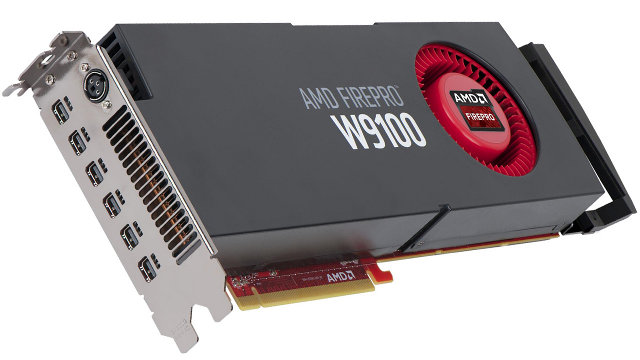
\includegraphics[width=0.99\textwidth]{figures/w9100.jpg} \\ AMD FirePro W9100 \\ 320 GB/sec
    \end{center}
   \end{minipage}
   \hspace{0.2cm}
%
   \begin{minipage}{0.3\textwidth}
    \begin{center}
     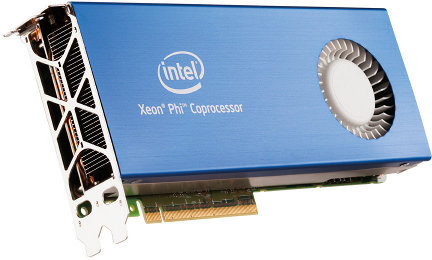
\includegraphics[width=0.92\textwidth]{figures/xeon-phi.jpg} \\ INTEL Xeon Phi \\ 320 (220?) GB/sec
    \end{center}
   \end{minipage}
   \hspace{0.2cm}
%
   \begin{minipage}{0.3\textwidth}
    \begin{center}
     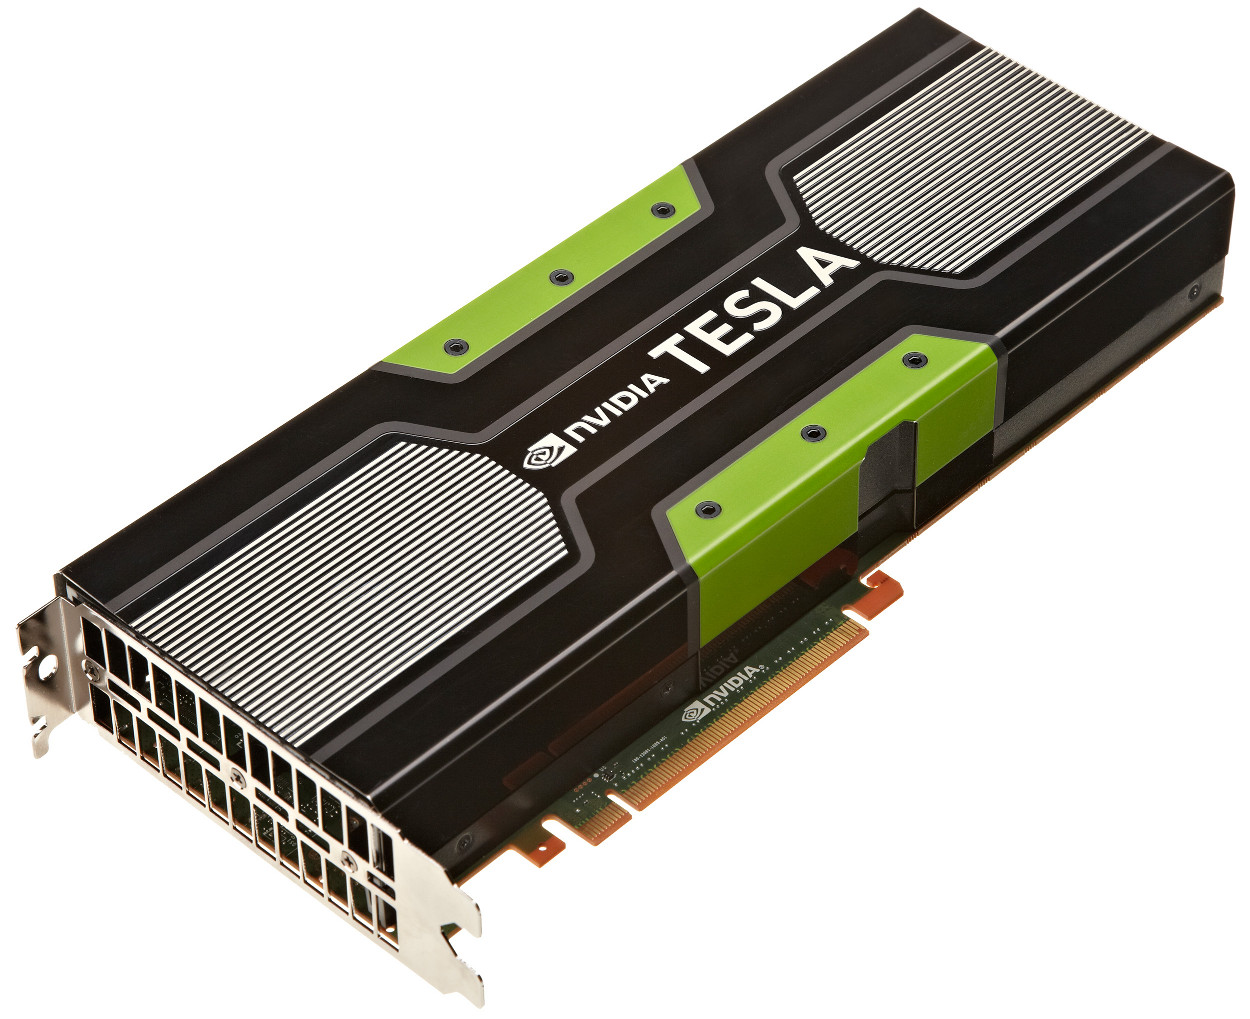
\includegraphics[width=0.7\textwidth]{figures/TeslaK20.jpg} \\ NVIDIA Tesla K20 \\ 250 (208) GB/sec
    \end{center}
   \end{minipage}


\end{frame}


\begin{frame}{Introduction}
 \vspace*{-0.5cm}
 \begin{center}
  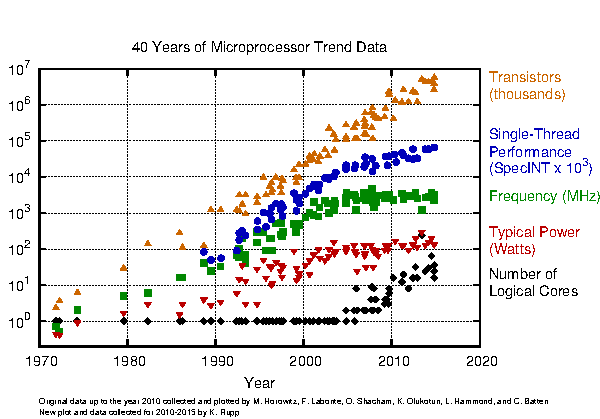
\includegraphics[width=0.95\textwidth]{figures/40-years-processor-trend}
 \end{center}
 {\tiny https://www.karlrupp.net/2015/06/40-years-of-microprocessor-trend-data/ }
\end{frame}

\begin{frame}{Introduction}
 \vspace*{-0.5cm}
 \begin{center}
  Theoretical Peak Performance \\
  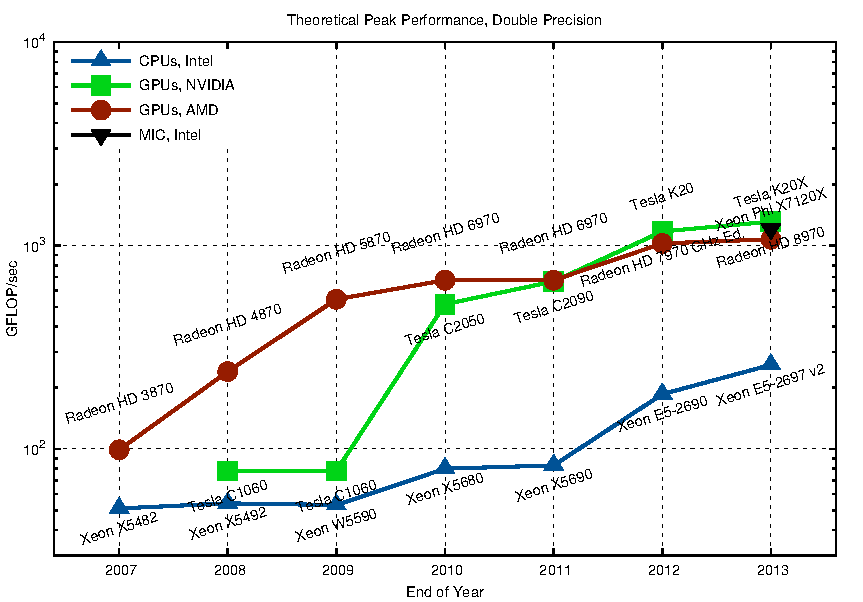
\includegraphics[width=0.95\textwidth]{figures/gflops-dp}
 \end{center}
 \vspace*{-0.5cm}
 {\tiny https://www.karlrupp.net/2013/06/cpu-gpu-and-mic-hardware-characteristics-over-time/ }
\end{frame}

\begin{frame}{Introduction}
 \vspace*{-0.5cm}
 \begin{center}
  Theoretical Peak Performance per Watt \\
  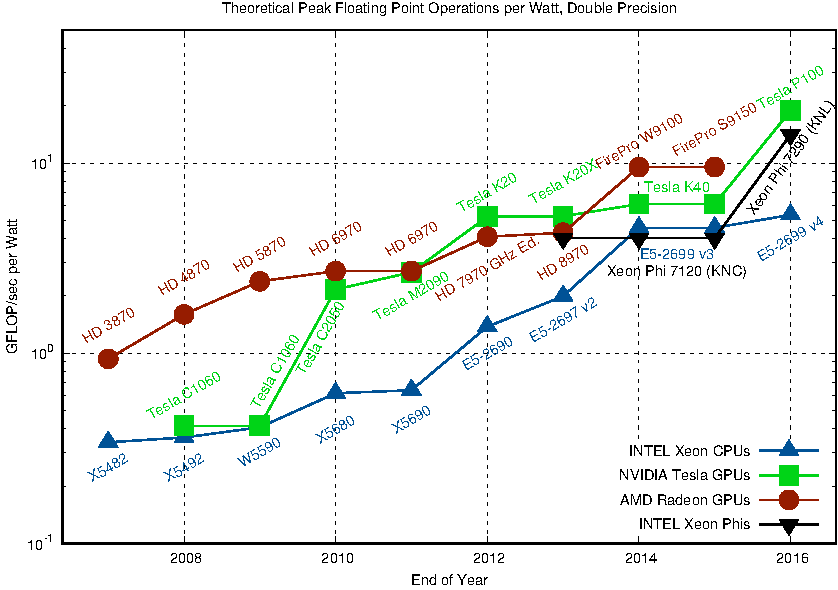
\includegraphics[width=0.95\textwidth]{figures/gflops-per-watt-dp}
 \end{center}
 \vspace*{-0.5cm}
 {\tiny https://www.karlrupp.net/2013/06/cpu-gpu-and-mic-hardware-characteristics-over-time/ }
\end{frame}

\begin{frame}{Introduction}
 \vspace*{-0.5cm}
 \begin{center}
  Theoretical Peak Performance (FLOPs) per Byte of Memory Bandwidth \\
  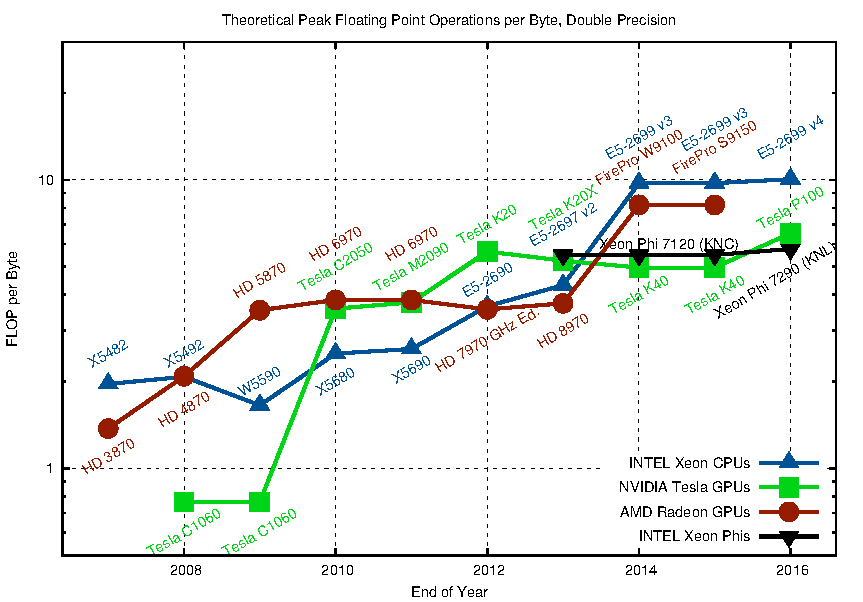
\includegraphics[width=0.95\textwidth]{figures/flop-per-byte-dp}
 \end{center}
 \vspace*{-0.5cm}
 {\tiny https://www.karlrupp.net/2013/06/cpu-gpu-and-mic-hardware-characteristics-over-time/ }
\end{frame}



%%
%%
%%  Part 1: ViennaCL
%%
%%



\begin{frame}{Contents}
  \begin{center}
   \Large Part 1: ViennaCL
  \end{center}
\end{frame}

\begin{frame}{Simulation Flow}
  \begin{center}
   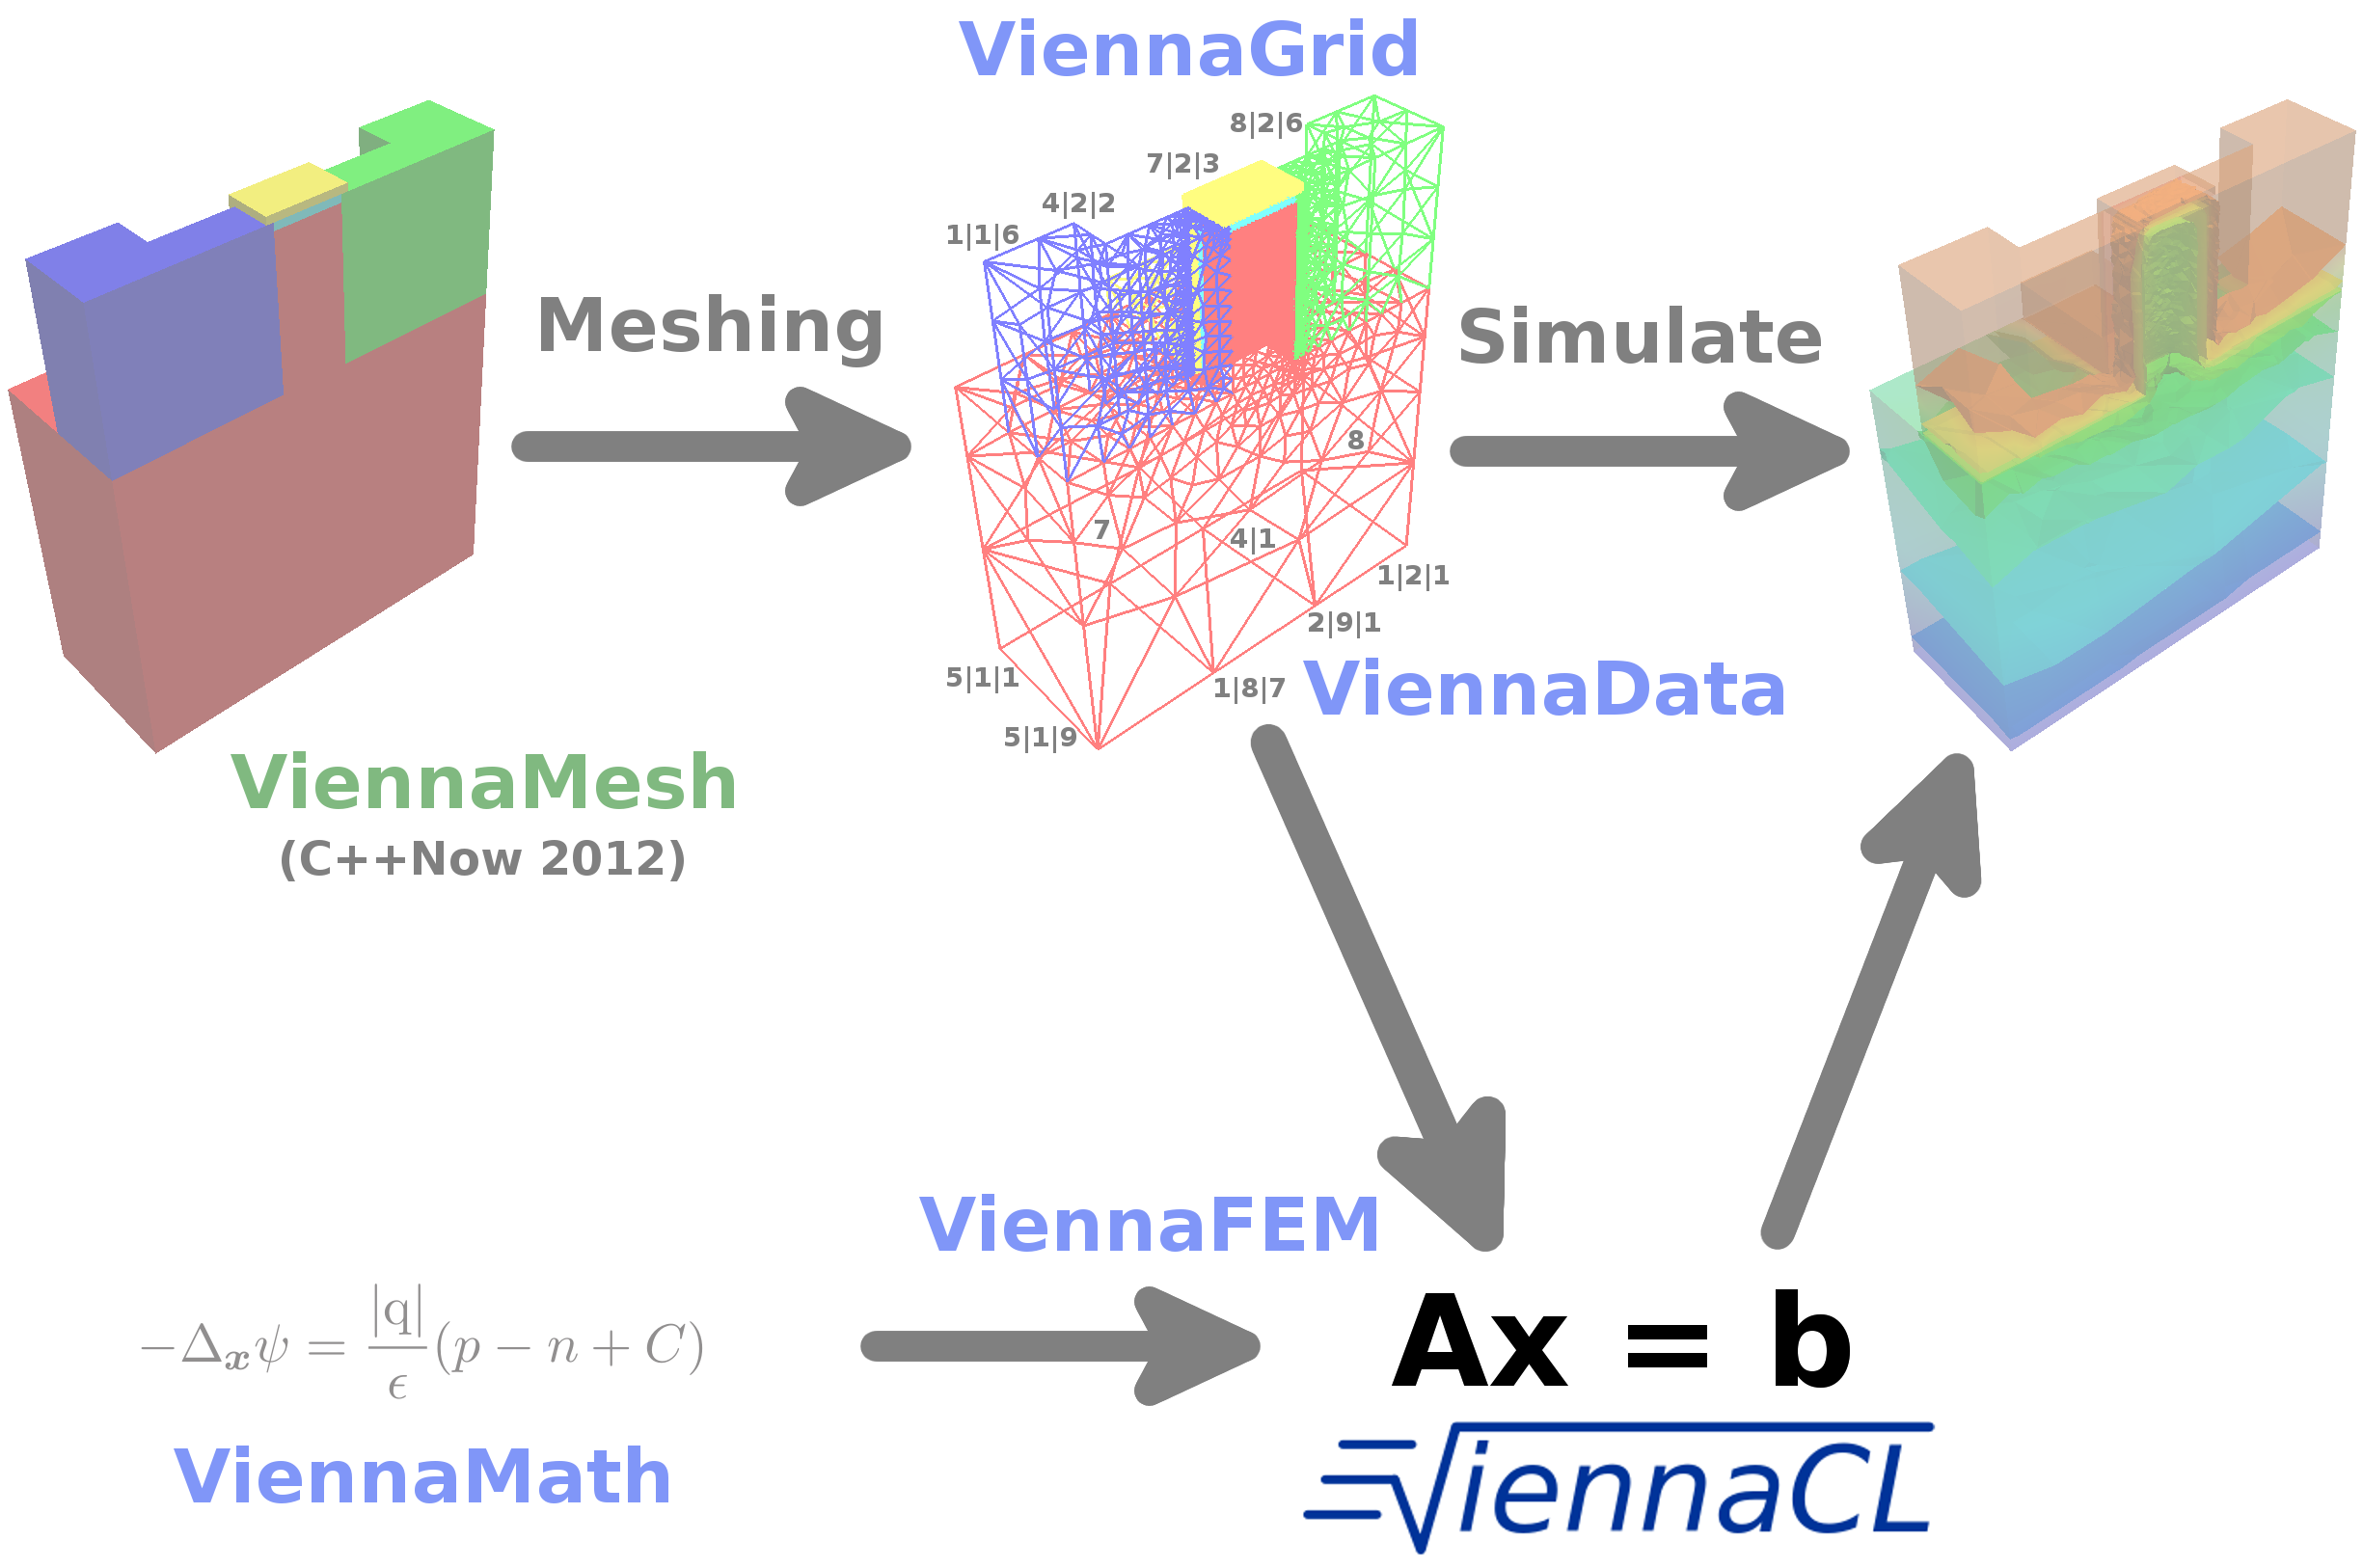
\includegraphics[width=0.99\textwidth]{flow-viennacl-2.png}
  \end{center}
\end{frame}



\begin{frame}[fragile]
\frametitle{From Boost.uBLAS to ViennaCL}
\begin{block}{Consider Existing CPU Code (Boost.uBLAS)}
  \begin{lstlisting}
using namespace boost::numeric::ublas;


matrix<double> A(1000, 1000);
vector<double> x(1000), y(1000);

/* Fill A, x, y here */

double val = inner_prod(x, y);
y += 2.0 * x;
A += val * outer_prod(x, y);

x = solve(A, y, upper_tag()); // Upper tri. solver

std::cout << "  2-norm: " << norm_2(x) << std::endl;
std::cout << "sup-norm: " << norm_inf(x) << std::endl;
  \end{lstlisting}

  \begin{itemize}
   \item High-level code with syntactic sugar
  \end{itemize}

\end{block}

\end{frame}


\begin{frame}[fragile]
\frametitle{From Boost.uBLAS to ViennaCL}
 \begin{block}{Previous Code Snippet Rewritten with ViennaCL}
  \begin{lstlisting}
using namespace viennacl;
using namespace viennacl::linalg;

matrix<double> A(1000, 1000);
vector<double> x(1000), y(1000);

/* Fill A, x, y here */

double val = inner_prod(x, y);
y += 2.0 * x;
A += val * outer_prod(x, y);

x = solve(A, y, upper_tag()); // Upper tri. solver

std::cout << "  2-norm: " << norm_2(x) << std::endl;
std::cout << "sup-norm: " << norm_inf(x) << std::endl;
  \end{lstlisting} 

  \begin{itemize}
   \item High-level code with syntactic sugar
  \end{itemize}

 \end{block}

\end{frame}



%%%%%%%%%%%%%%% Iterative solvers %%%%%%%%%%%%%%%%%%%%%%
\begin{frame}[fragile]
\frametitle{From Boost.uBLAS to ViennaCL}
\begin{block}{ViennaCL in Addition Provides Iterative Solvers}
  \begin{lstlisting}
using namespace viennacl;
using namespace viennacl::linalg;

compressed_matrix<double> A(1000, 1000);
vector<double> x(1000), y(1000);

/* Fill A, x, y here */

x = solve(A, y, cg_tag());       // Conjugate Gradients
x = solve(A, y, bicgstab_tag()); // BiCGStab solver
x = solve(A, y, gmres_tag());    // GMRES solver
  \end{lstlisting}
\end{block}

 \begin{block}{No Iterative Solvers Available in Boost.uBLAS...}
  \vspace*{1.22cm}
 \end{block}
\end{frame}


\begin{frame}[fragile]
\frametitle{From Boost.uBLAS to ViennaCL}
\begin{block}{Thanks to Interface Compatibility}
  \begin{lstlisting}
using namespace boost::numeric::ublas;
using namespace viennacl::linalg;

compressed_matrix<double> A(1000, 1000);
vector<double> x(1000), y(1000);

/* Fill A, x, y here */

x = solve(A, y, cg_tag());       // Conjugate Gradients
x = solve(A, y, bicgstab_tag()); // BiCGStab solver
x = solve(A, y, gmres_tag());    // GMRES solver
  \end{lstlisting} 
\end{block}

\begin{block}{Code Reuse Beyond GPU Borders}
 \begin{itemize}
  \item Eigen \ { \ \footnotesize \verb|http://eigen.tuxfamily.org/|}
  \item MTL 4 \ { \footnotesize \verb|http://www.mtl4.org/|}
 \end{itemize}
\end{block}

\end{frame}





\begin{frame}{About ViennaCL}

  \begin{block}{About}
   \begin{itemize}
    \item High-level linear algebra C++ library
    \item OpenMP, OpenCL, and CUDA backends
    \item Header-only
    \item Multi-platform
   \end{itemize}
  \end{block}

  \vspace*{-2.3cm}
  \begin{flushright}
   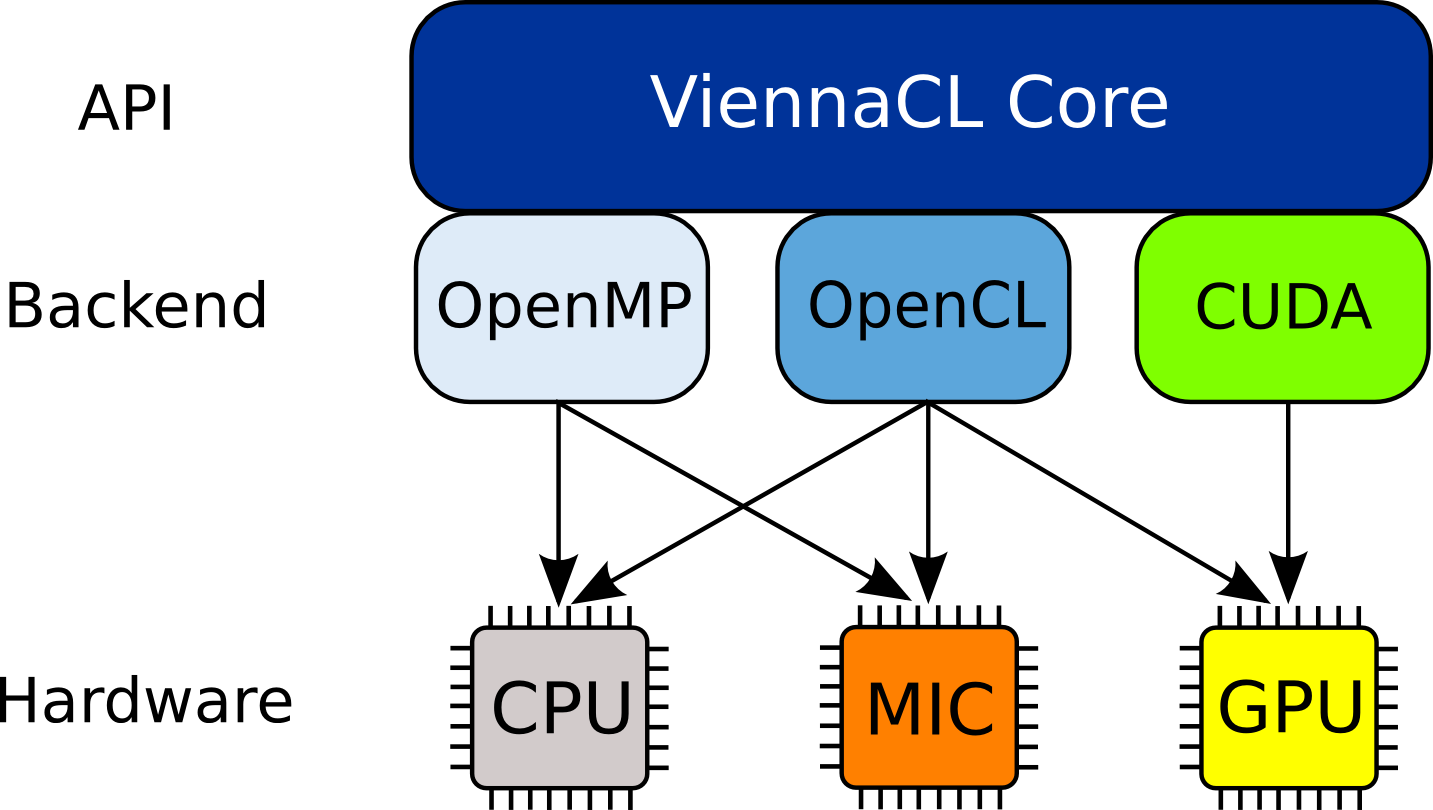
\includegraphics[width=0.4\textwidth]{figures/ViennaCL-arch.png}
  \end{flushright}

  \vspace*{-0.7cm}
  \begin{block}{Dissemination}
    \begin{itemize}
     \item Free Open-Source MIT (X11) License
     \item http://viennacl.sourceforge.net/
     \item 50-100 downloads per week
    \end{itemize}   
  \end{block}

  \begin{block}{Design Rules}
   \begin{itemize}
    \item Reasonable default values
    \item Compatible to Boost.uBLAS whenever possible 
    \item In doubt: clean design over performance
   \end{itemize}
  \end{block}

\end{frame}



\begin{frame}[fragile]
\frametitle{About ViennaCL}

 \begin{block}{Basic Types}
   \begin{itemize}
    \item scalar, vector
    \item matrix, compressed\_matrix, coordinate\_matrix, ell\_matrix, hyb\_matrix
   \end{itemize}
 \end{block}

 \begin{block}{Data Initialization}
    \begin{itemize}
    \item  { 
  \begin{lstlisting}
     std::vector<double>      std_x(100);
   ublas::vector<double>    ublas_x(100);
viennacl::vector<double>      vcl_x(100);

for (size_t i=0; i<100; ++i)
  //   std_x[i] = rand();  // (1)
  // ublas_x[i] = rand();  // (2)
       vcl_x[i] = rand();  // (3)

  \end{lstlisting} }
    \item (3) is fastest, right?
%   \item Reuse of C++ STL coding conventions
 \end{itemize}

 \end{block}
\end{frame}





\begin{frame}[fragile]
\frametitle{About ViennaCL}

 \begin{block}{Basic Types}
   \begin{itemize}
    \item scalar, vector
    \item matrix, compressed\_matrix, coordinate\_matrix, ell\_matrix, hyb\_matrix
   \end{itemize}
 \end{block}

 \begin{block}{Data Initialization}
    \begin{itemize}
     \item Using viennacl::copy() 
    \item  { 
  \begin{lstlisting}
     std::vector<double>      std_x(100);
   ublas::vector<double>    ublas_x(100);
viennacl::vector<double>      vcl_x(100);

/* setup of std_x and ublas_x omitted */

viennacl::copy(std_x.begin(), std_x.end(),
               vcl_x.begin());   //to GPU
viennacl::copy(vcl_x.begin(), vcl_x.end(),
               ublas_x.begin()); //to CPU
  \end{lstlisting} }

 \end{itemize}

 \end{block}
\end{frame}


\begin{frame}[fragile]
\frametitle{About ViennaCL}

 \begin{block}{Basic Types}
   \begin{itemize}
    \item scalar, vector
    \item matrix, compressed\_matrix, coordinate\_matrix, ell\_matrix, hyb\_matrix
   \end{itemize}
 \end{block}

 \begin{block}{Data Initialization}
    \begin{itemize}
     \item Using viennacl::copy() 
    \item  { 
  \begin{lstlisting}
     std::vector<std::vector<double> >    std_A;
   ublas::matrix<double>                ublas_A;
viennacl::matrix<double>                  vcl_A;

/* setup of std_A and ublas_A omitted */

viennacl::copy(std_A, vcl_A);    // CPU to GPU
viennacl::copy(vcl_A, ublas_A);  // GPU to CPU
  \end{lstlisting} }
    \item Iterator concept doesn't quite work on accelerators
 \end{itemize}

 \end{block}
\end{frame}





\begin{frame}[fragile]
\frametitle{Internals}

 \begin{block}{Vector Addition}
  \begin{lstlisting}
 x = y + z;
  \end{lstlisting}
  
  \begin{itemize}
   \item Temporaries are costly (particularly on GPUs)
  \end{itemize}

 \end{block}


 \begin{block}{Expression Templates}
  \begin{itemize}
   \item Limited expansion
   \item Map to a set of predefined kernels
  \end{itemize}
  
  \begin{lstlisting}
 vector_expression<vector<T>, op_plus, vector<T> >
 operator+(vector<T> & v, vector<T> & w) { ... }

 vector::operator=(vector_expression<...> const & e) {
   viennacl::linalg::avbv(*this, 1,e.lhs(), 1,e.rhs());
 }
  \end{lstlisting}
  \vspace*{0.5cm}

 \end{block}

\end{frame}



\begin{frame}[fragile]
\frametitle{Internals}

 \begin{block}{Vector Addition}
  \begin{lstlisting}
// x = y + z
void avbv(...) {
  switch (active_handle_id(x)) {
    case MAIN_MEMORY:
      host_based::avbv(...);
      break;
    case OPENCL_MEMORY:
      opencl::avbv(...);
      break;
    case CUDA_MEMORY:
      cuda::avbv(...);
      break;
    default: 
      raise_error();
  }
}
\end{lstlisting}
  \begin{itemize}
   \item Memory buffers can switch memory domain at runtime
  \end{itemize}

 \end{block}

\end{frame}

\begin{frame}[fragile]
\frametitle{Internals}

 \begin{block}{Memory Buffer Migration}
  \begin{lstlisting}
  vector<double> x = zero_vector<double>(42);

  memory_types src_memory_loc = memory_domain(x);
  switch_memory_domain(x, MAIN_MEMORY);

  /* work on x in main memory here */

  switch_memory_domain(x, src_memory_loc);
\end{lstlisting}

  \begin{center}
    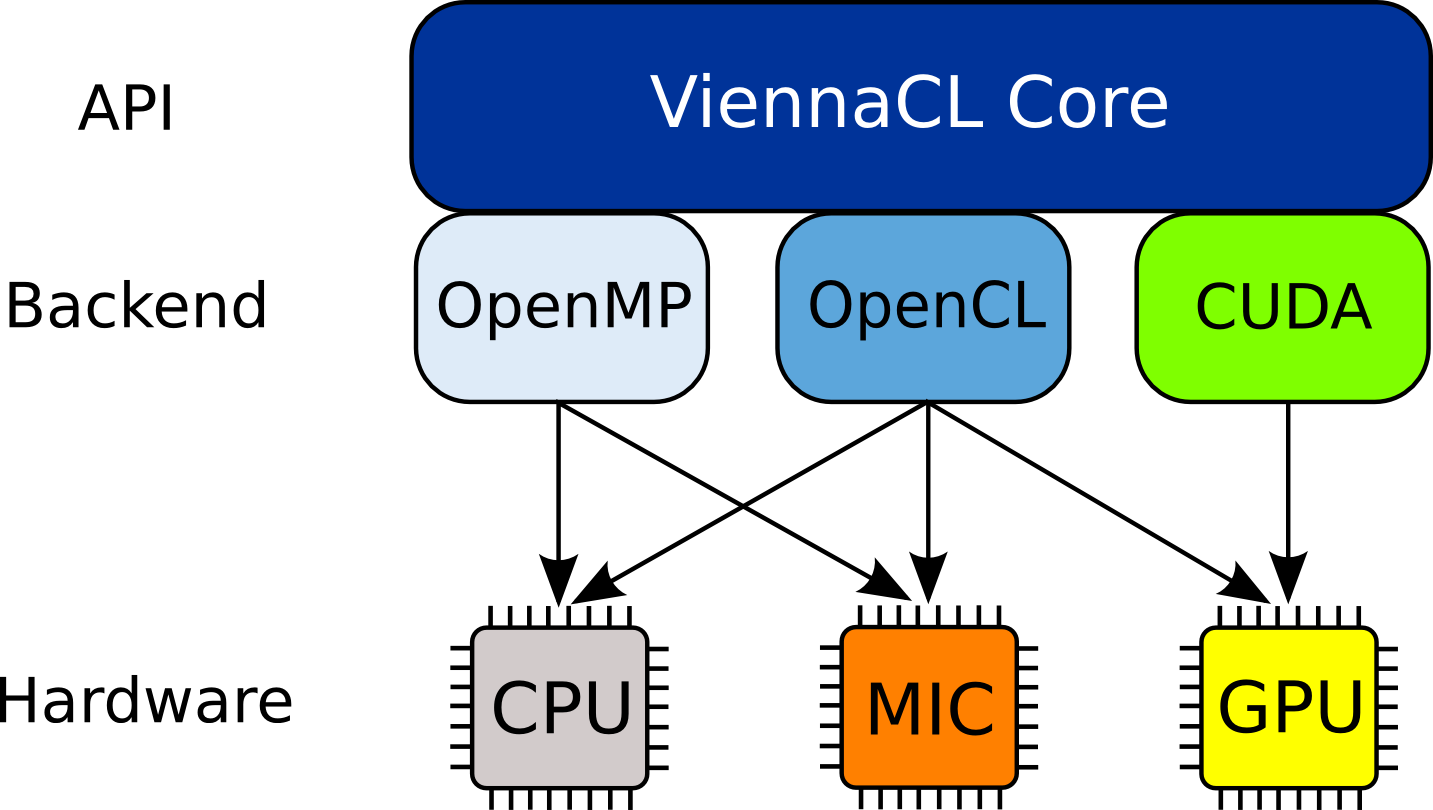
\includegraphics[width=0.5\textwidth]{figures/ViennaCL-arch.png}
  \end{center}
 \end{block}

\end{frame}




\begin{frame}[fragile]
\frametitle{Internals}

 \begin{block}{Generalizing compute kernels}
  \begin{lstlisting}
  // x = y + z
  __kernel void avbv(
    double * x,

    double * y,

    double * z, uint size)
{
  size_t i = get_global_id(0);
  for (; i<size; i += get_global_size())
    x[i] = y[i] + z[i]; 

}
  \end{lstlisting}
 \end{block}

 \vspace*{1.57cm}
\end{frame}



\begin{frame}[fragile]
\frametitle{Internals}

 \begin{block}{Generalizing compute kernels}
  \begin{lstlisting}
  // x = a * y + b * z
  __kernel void avbv(
    double * x,
    double a,
    double * y,
    double b,
    double * z, uint size)
{
  size_t i = get_global_id(0);
  for (; i<size; i += get_global_size())
    x[i] = a * y[i] + b * z[i]; 

}
  \end{lstlisting}
 \end{block}

 \vspace*{1.57cm}
\end{frame}


\begin{frame}[fragile]
\frametitle{Internals}

 \begin{block}{Generalizing compute kernels}
  \begin{lstlisting}
  // x[4:8] = a * y[2:6] + b * z[3:7]
  __kernel void avbv(
    double * x, uint off_x,
    double a,
    double * y, uint off_y,
    double b,
    double * z, uint off_z, uint size)
{
  size_t i = get_global_id(0);
  for (; i<size; i += get_global_size())
    x[off_x + i] = a * y[off_y + i] + b * z[off_z + i]; 

}
  \end{lstlisting}
 \end{block}

 \vspace*{1.57cm}
\end{frame}



\begin{frame}[fragile]
\frametitle{Internals}

 \begin{block}{Generalizing compute kernels}
  \begin{lstlisting}
  // x[4:2:8] = a * y[2:2:6] + b * z[3:2:7]
  __kernel void avbv(
    double * x, uint off_x, uint inc_x,
    double a,
    double * y, uint off_y, uint inc_y,
    double b,
    double * z, uint off_z, uint inc_z, uint size)
{
  size_t i = get_global_id(0);
  for (; i<size; i += get_global_size())
    x[off_x + i * inc_x] =  a * y[off_y + i * inc_y]
                          + b * z[off_z + i * inc_z]; 
}
  \end{lstlisting}
 \end{block}

  \begin{block}{}
   \begin{itemize}
    \item No penalty on NVIDIA GPUs because FLOPs are for free
   \end{itemize}
  \end{block}

\end{frame}






\begin{frame}{Benchmarks}
  \begin{center}
   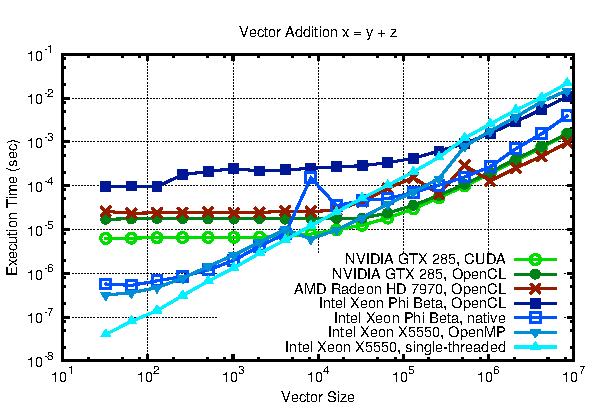
\includegraphics[width=0.95\textwidth]{figures/vector-timings-7}
  \end{center}
\end{frame}

%%


\begin{frame}{Benchmarks}
  \begin{center}
   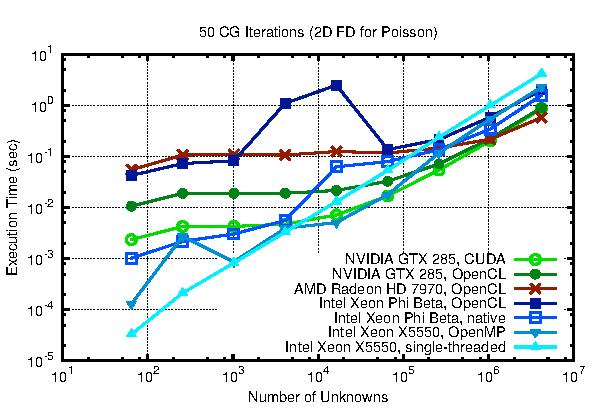
\includegraphics[width=0.95\textwidth]{figures/cg-timings-7}
  \end{center}
\end{frame}




%%%%%%%%%%%%%%%%%%%%%%%%%%%%%%%%%%%%%%%%%


\begin{frame}{Benchmarks}

 \begin{block}{Matrix-Matrix Multiplication}
  \begin{itemize}
   \item Autotuning environment 
   \item 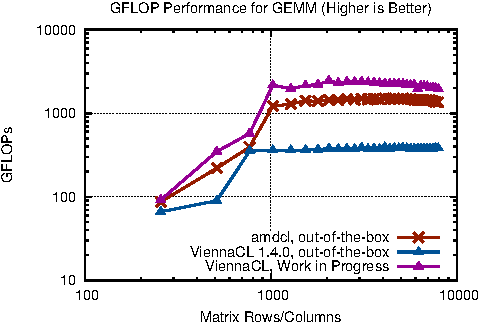
\includegraphics[width=0.8\textwidth]{figures/gemm3.pdf}
   \item \centering (AMD Radeon HD 7970, single precision)
  \end{itemize}

 \end{block}

\end{frame}





\begin{frame}[fragile]{Expression Template Limitations}

 \begin{block}{Expression Templates are Not Enough}
  \begin{itemize}
   \item Consider
    \begin{lstlisting}
     u = x + y;
     v = x - y;
    \end{lstlisting}
   \item Suboptimal performance with almost any library
  \end{itemize}
 \end{block}
 
 \begin{center}
  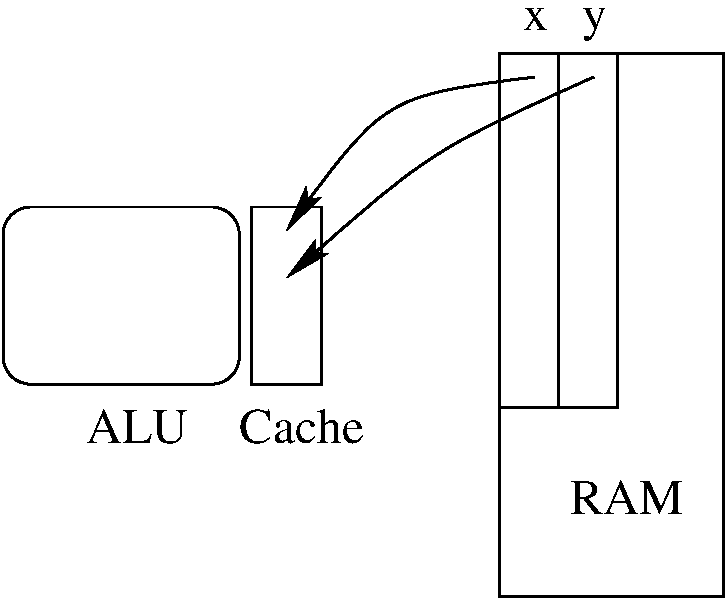
\includegraphics[width=0.4\textwidth]{kernel-fusion-1.pdf}
 \end{center}


\end{frame}



\begin{frame}[fragile]{Expression Template Limitations}

 \begin{block}{Expression Templates are Not Enough}
  \begin{itemize}
   \item Consider
    \begin{lstlisting}
     u = x + y;
     v = x - y;
    \end{lstlisting}
   \item Suboptimal performance with almost any library
  \end{itemize}
 \end{block}
 
 \begin{center}
  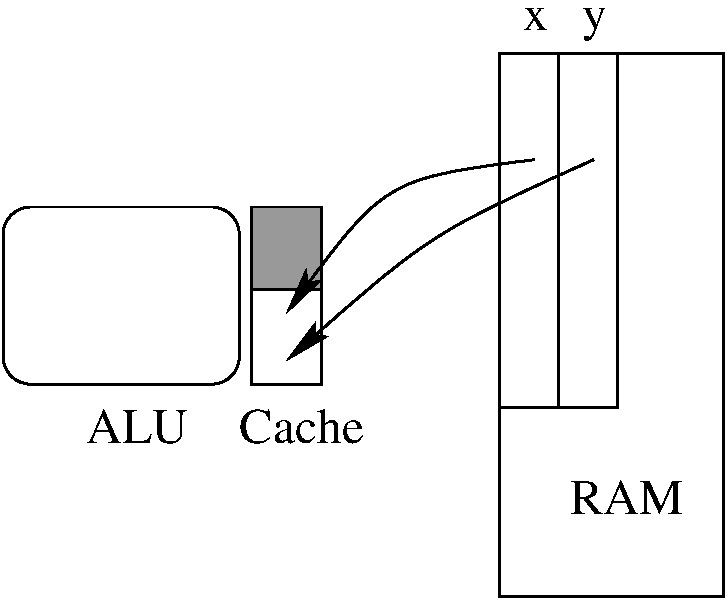
\includegraphics[width=0.4\textwidth]{kernel-fusion-2.pdf}
 \end{center}


\end{frame}


\begin{frame}[fragile]{Expression Template Limitations}

 \begin{block}{Expression Templates are Not Enough}
  \begin{itemize}
   \item Consider
    \begin{lstlisting}
     u = x + y;
     v = x - y;
    \end{lstlisting}
   \item Suboptimal performance with almost any library
  \end{itemize}
 \end{block}

 \begin{block}{OpenCL Kernel Generation}
   \begin{itemize}
    \item Separate temporary avoidance from operation execution
    \begin{lstlisting}
      custom_operation op;
      op.add( u = x + y );
      op.add( v = x - y );
      op.execute();          // OpenCL JIT
    \end{lstlisting}
    \item Fully transparent kernel fusion scheduled for release 1.5.0
   \end{itemize}
 \end{block}
\end{frame}


\begin{frame}{Expression Template Limitations}

 \begin{block}{Benchmark Results}
  \begin{center}
   $\beta \leftarrow x^T \cdot (2x + y)$ \\
   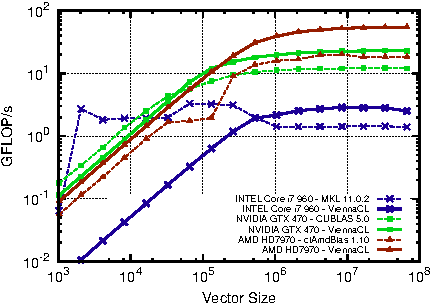
\includegraphics[width=0.75\textwidth]{figures/daxpy_ddot.pdf} \\
  \end{center}
   \scriptsize Tillet \textit{et al.}, HotPar '13

 \end{block}

\end{frame}






%%
%%
%%  Part 2: ViennaGrid
%%
%%



\begin{frame}{Contents}
  \begin{center}
   \Large Part 2: ViennaGrid
  \end{center}
\end{frame}

\begin{frame}{Simulation Flow}
  \begin{center}
   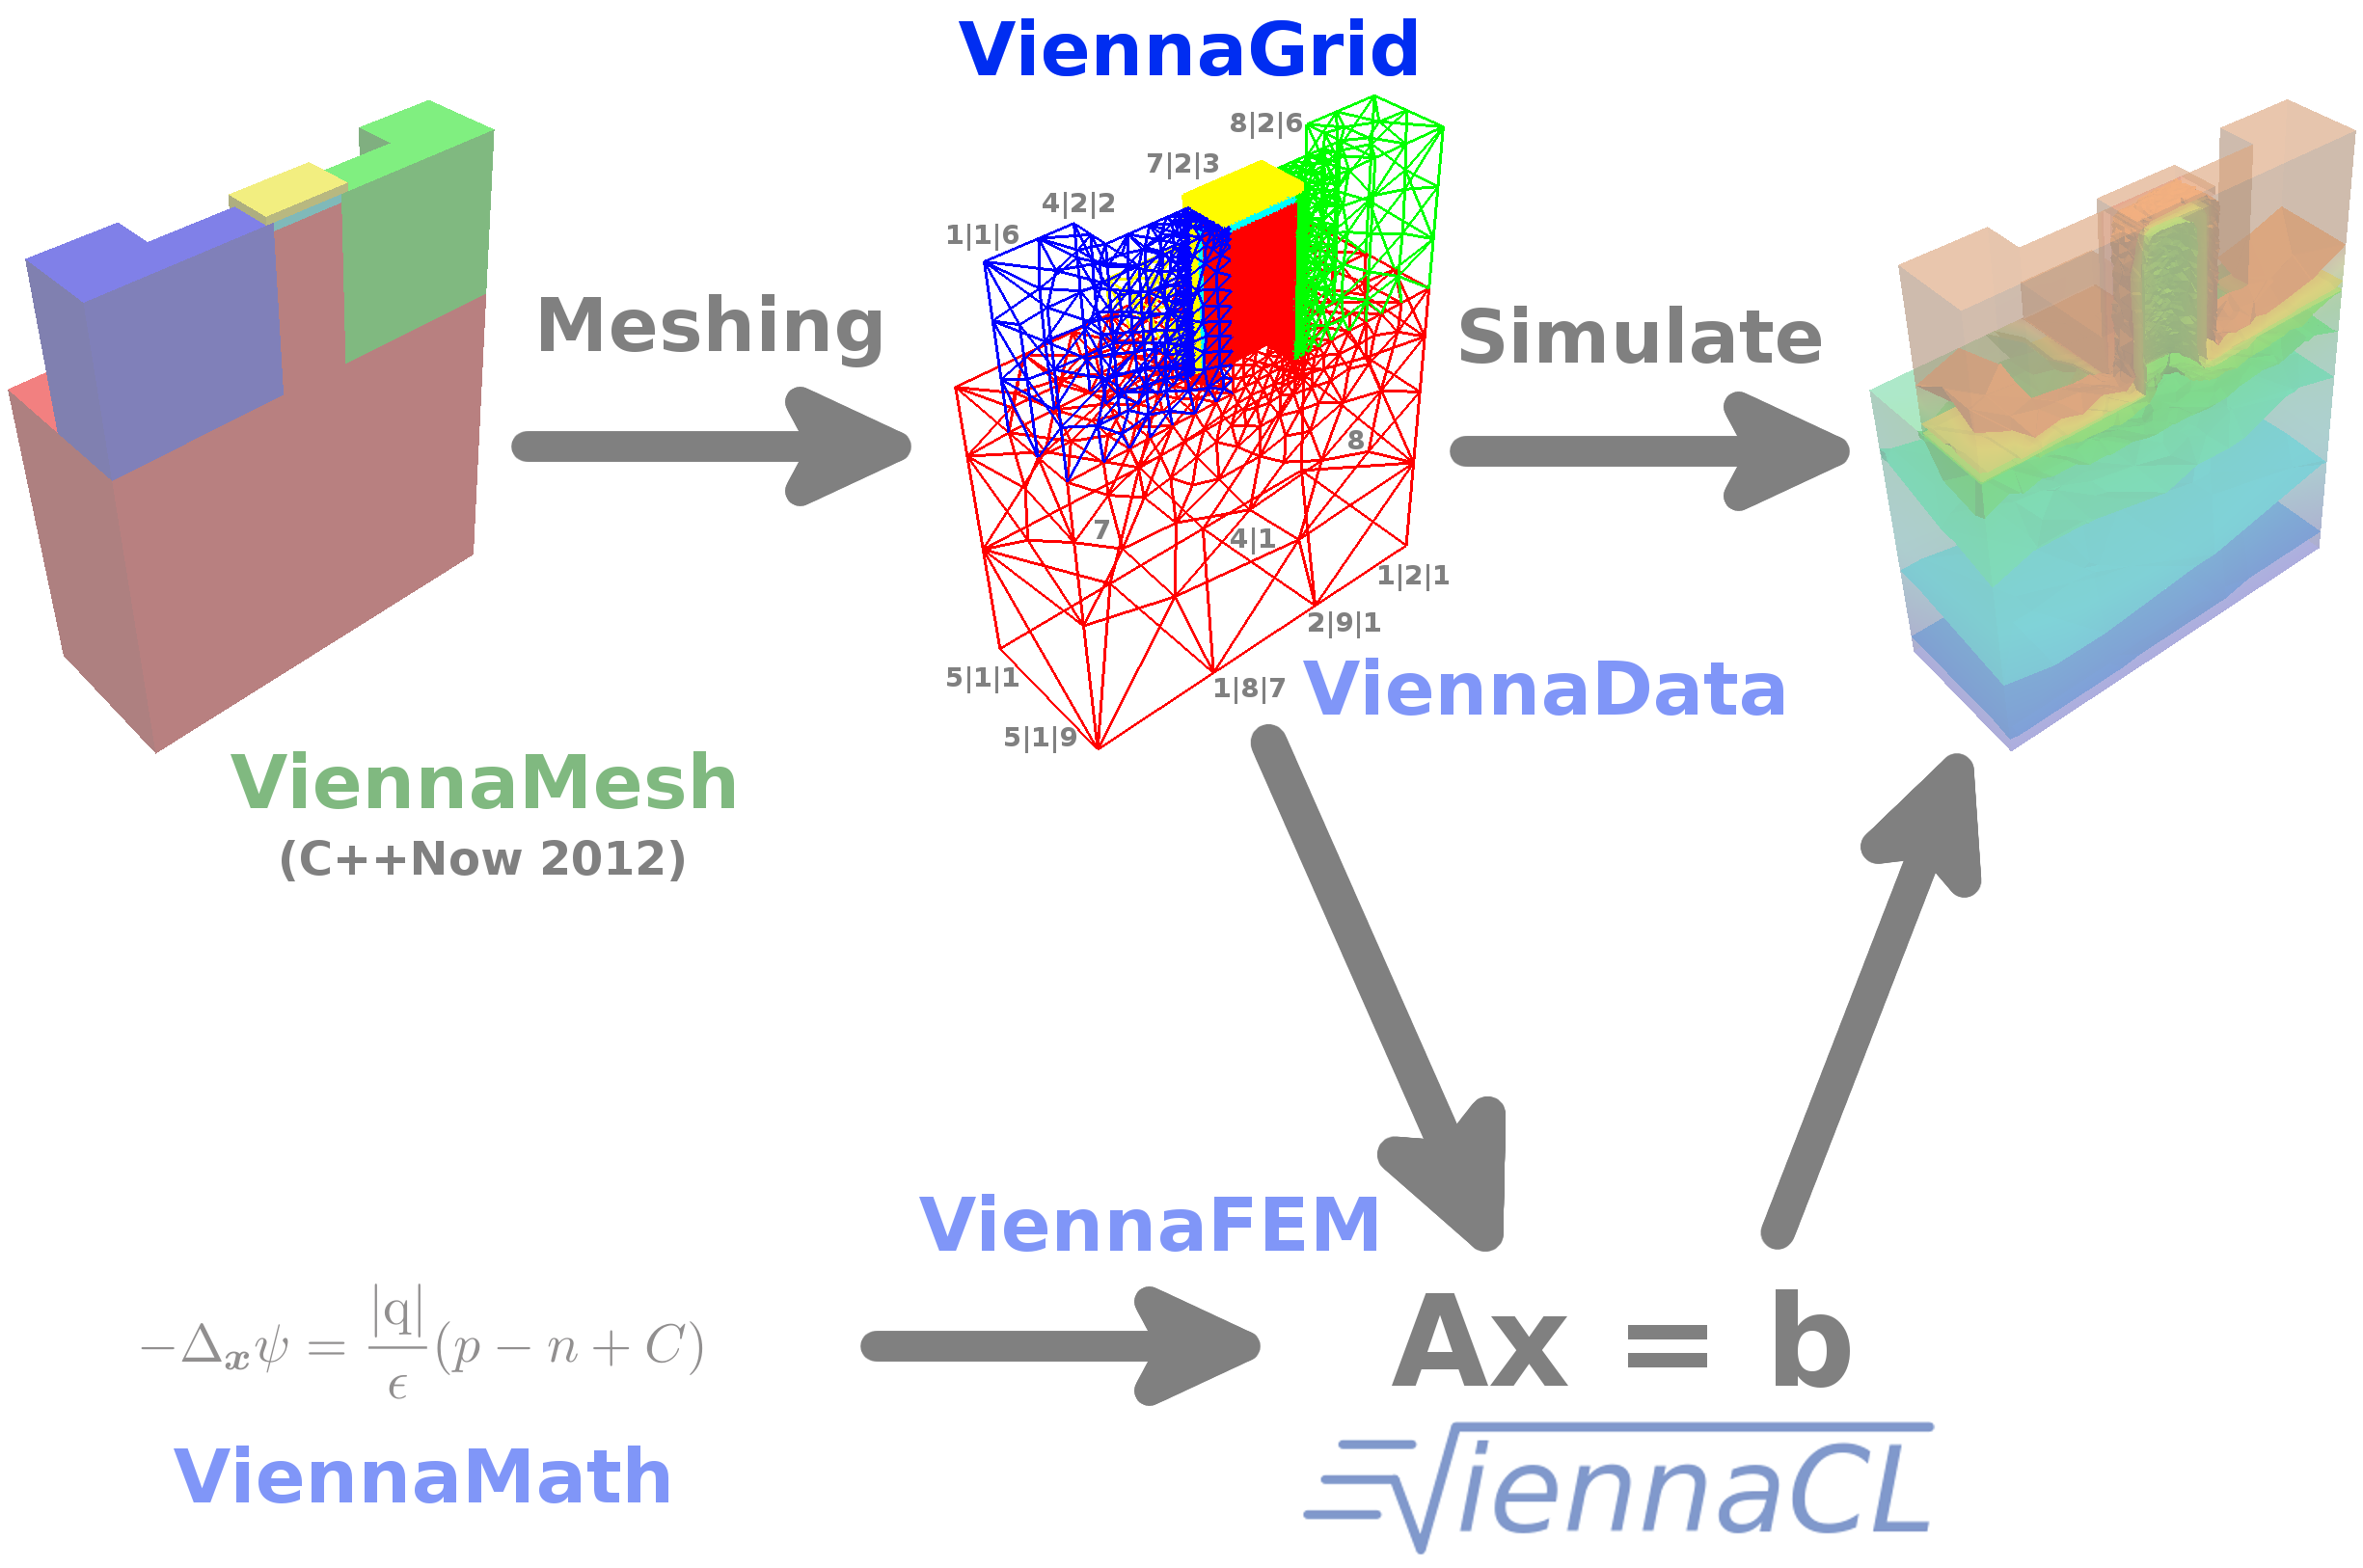
\includegraphics[width=0.99\textwidth]{flow-viennagrid-2.png}
  \end{center}
\end{frame}





% Quick look: Boost Geometry
\begin{frame}[fragile]{What about Boost.Geometry?}
 \begin{block}{A Quick Look at Boost.Geometry}
  \begin{itemize}
   \item Concepts: Point, Segment, Linestring, Box, etc.
   \item Algorithms: \lstinline|distance()|, \lstinline|intersects()|, \lstinline|convex_hull()|, etc.
   \item Central entity: Point
  \end{itemize}
  \begin{lstlisting}
   int a[3] = {1, 2, 3};
   int b[3] = {2, 3, 4};

   double d = boost::geometry::distance(a, b);
  \end{lstlisting}  
 \end{block}

 \visible<1->{
 \begin{block}{Why Boost.Geometry is Not Enough}
  \begin{itemize}
   \item What about 3D objects? Tetrahedra? Hexahedra?
   \item Traversal of boundary objects missing
   \item No storage facilities for \emph{many} objects
  \end{itemize}
 \end{block}
 }
\end{frame}






% Introduce Topology

\begin{frame}{$n$-cell Concept}
 \begin{block}{Concept of \emph{$n$-cell}}
  \begin{itemize}
   \item Sub-$k$-cells of an $n$-cell
  \end{itemize}
  \vspace*{-0.3cm}
  \begin{center}
    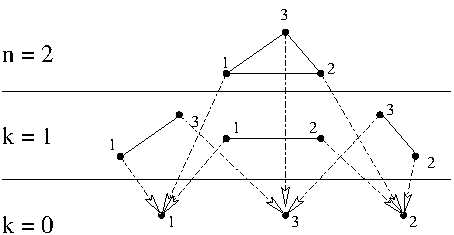
\includegraphics[width=0.37\textwidth]{triangle-layers} \hspace{0.2cm}
    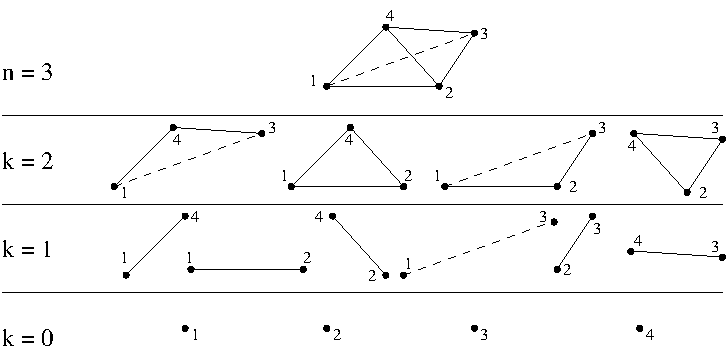
\includegraphics[width=0.59\textwidth]{tetrahedron-layers}
  \end{center}
 \end{block}

 \visible<1->{
 \begin{block}{Separation of Geometry and Topology}
  \begin{itemize}
    \item Geometry: Euclidian space, coordinate system
    \item Topology: Connection between points (lines, triangles, etc.)
  \end{itemize}
 \end{block}
 \vspace*{0.3cm}
 }
\end{frame}




\begin{frame}[fragile]
\frametitle{ViennaGrid Datastructure}
 \begin{block}{Datastructure Requirements}
   \begin{itemize}
    \item Don't store boundary $k$-cells unnecessarily
    \item Fast local iteration on $k$-cells
   \end{itemize}
 \end{block}

  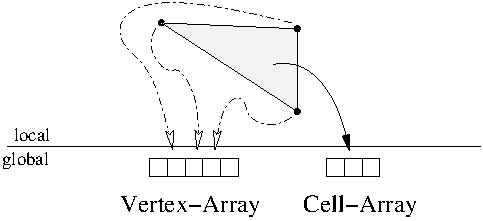
\includegraphics[width=0.45\textwidth]{storage-vglob-cglob} \hspace*{0.3cm}
  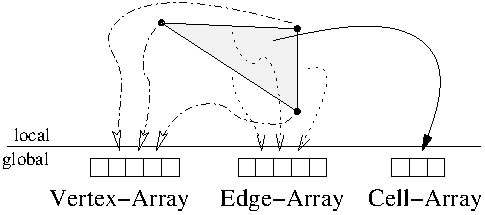
\includegraphics[width=0.49\textwidth]{storage-vglob-eglob-cglob} \\

 \visible<1->{
 \vspace*{0.3cm} 
 \begin{tabular}{|l|r|r|r|}
  \hline
         & \scriptsize Amount      & \scriptsize Mem/Obj.         & \scriptsize Total Mem. \\
  \hline
  \tiny Vertices & \footnotesize 4913 & \footnotesize 24 B & \footnotesize 115 KB \\
  \hline
  \tiny Edges   & \footnotesize 31024 & \footnotesize 16 B & \footnotesize 485 KB \\
  \hline
  \tiny Facets  & \footnotesize 50688 & \footnotesize 48 B & \footnotesize 2376 KB \\
  \hline
  \tiny Cells   & \footnotesize 24576 & \footnotesize 112 B & \footnotesize 2688 KB \\
  \hline
  \scriptsize \textbf{Total}  &       &     & \footnotesize  \textbf{5664 KB} \\
  \hline
 \end{tabular}
 \begin{tabular}{|l|r|r|r|}
  \hline
         & \scriptsize Amount      & \scriptsize Mem/Obj.         & \scriptsize Total Mem. \\
  \hline
  \tiny Vertices & \footnotesize 4913 & \footnotesize 24 B & \footnotesize 115 KB \\
  \hline
  \tiny Edges   & \footnotesize 0 & - & \footnotesize 0 KB \\
  \hline
  \tiny Facets  & \footnotesize 0 & - & \footnotesize 0 KB \\
  \hline
  \tiny Cells   & \footnotesize 24576 & \footnotesize 32 B & \footnotesize 768 KB \\
  \hline
  \scriptsize \textbf{Total}  &       &     & \footnotesize  \textbf{883 KB} \\
  \hline
 \end{tabular}
 \vspace*{0.5cm}
 }
\end{frame}




\begin{frame}[fragile]{$n$-cell Implementation}

 \begin{block}{Implementation of \lstinline|element_t|}
  \begin{itemize}
   \item Recursive inheritance from boundary layer of dimension $n-1$
   \item Tag dispatching to enable/disable topological layers
  \end{itemize}
  \vspace*{-0.2cm}
  \begin{center}
    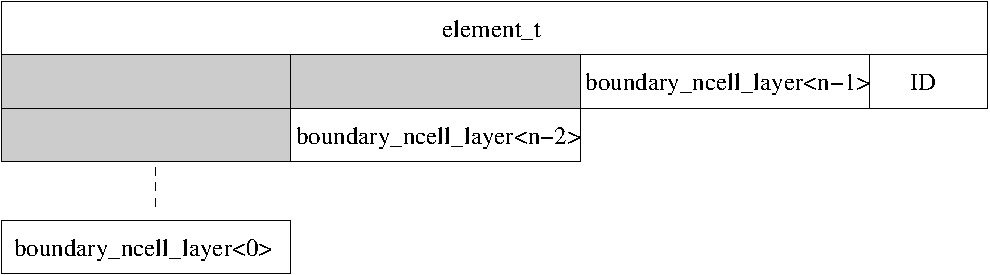
\includegraphics[width=0.77\textwidth]{recursive-inheritance}
  \end{center}
 \end{block}

 %\visible<2->{
 \begin{lstlisting}[basicstyle=\scriptsize\ttfamily]
  template <typename ConfigType, typename ElementTag>
  class element_t :
    public boundary_ncell_layer<ConfigType, ElementTag, ElementTag::dim-1>,
    public result_of::element_id_handler<ConfigType, ElementTag>::type
 \end{lstlisting}
 \vspace*{0.3cm}
 %}
\end{frame}





\begin{frame}[fragile]
\frametitle{Domain Configuration}
 \begin{block}{Top Level Configuration of Domain}
  \begin{itemize}
   \item Mostly a collection of tags
   \item Predefined configuration classes for common cases
   \item ViennaGrid 1.0.x: Supplemented by global customizations
  \end{itemize}

  \begin{lstlisting}
   struct triangular_3d
   {
     typedef double            numeric_type;
     typedef cartesian_cs<3>   coordinate_system_tag;
     typedef triangle_tag      cell_tag;
   };
   
   result_of::domain<triangular_3d>::type     Domain;
  \end{lstlisting} 

  \begin{itemize}
   \item Work in progress: Everything in a single config class
  \end{itemize}
 \end{block}
 \vspace*{0.45cm}
\end{frame}








\begin{frame}[fragile]
\frametitle{ViennaGrid User API}
 \begin{block}{User API Design Goals}
  \begin{itemize}
   \item STL-style, reuse conventions
   \item Allow index-based traversal
   \item Avoid common C++ pitfalls (e.g.~template member functions)
  \end{itemize}

  \begin{lstlisting}[basicstyle=\scriptsize\ttfamily,escapechar=@]
  //iteration over all vertices in the domain:
  typedef result_of::ncell_range<@\color{red}DomainType@, @\color{red}0@>::type  VertexRange;
  typedef result_of::iterator<VertexRange>::type       VertexIterator;
  
  VertexRange vertices = ncells<@\color{red}0@>(@\color{red}domain@);
  for (VertexIterator it  = vertices.begin();
                      it != vertices.end();
                    ++it)
  {
    // do something with each vertex here
  }
  \end{lstlisting} 

   \begin{itemize}
    \item \emph{Ranges} provide iterators over $n$-cells
    \item Extendible
   \end{itemize}
 \end{block}
 \vspace*{0.45cm}
\end{frame}


\begin{frame}[fragile]
\frametitle{ViennaGrid User API}
 \begin{block}{User API Design Goals}
  \begin{itemize}
   \item STL-style, reuse conventions
   \item Allow index-based traversal
   \item Avoid common C++ pitfalls (e.g.~template member functions)
  \end{itemize}

  \begin{lstlisting}[basicstyle=\scriptsize\ttfamily,escapechar=@]
  //iteration over all vertices in the domain:
  
  for (std::size_t i = 0; i < ncells<@\color{red}0@>(@\color{red}domain@).size(); ++i)
  {
    // do something with ncells<0>(domain)[i] here
  }
  \end{lstlisting} 

   \begin{itemize}
    \item OpenMP friendly
    \item \lstinline|.size()| sometimes known at compiletime!
   \end{itemize}
 \end{block}
 \vspace*{1.75cm}
\end{frame}

 
\begin{frame}[fragile]
\frametitle{ViennaGrid User API}
 \begin{block}{User API Design Goals}
  \begin{itemize}
   \item Boundary iteration: $k < n$
   \item Coboundary iteration: $k > n$
  \end{itemize}
  
  \begin{flushright}
   \vspace*{-2cm}
   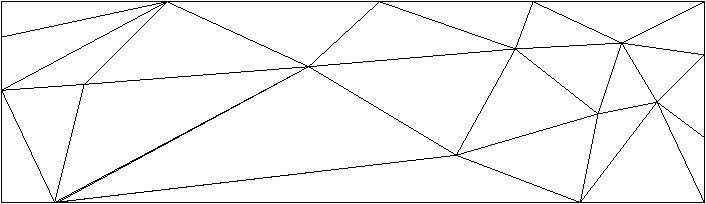
\includegraphics[width=0.5\textwidth]{figures/mesh.pdf}
  \end{flushright}


  \begin{lstlisting}[basicstyle=\scriptsize\ttfamily,escapechar=@]
  //iteration over all triangles of a vertex
  typedef result_of::ncell_range<@\color{red}VertexType@, @\color{red}2@>::type  TriangleRange;
  typedef result_of::iterator<TriangleRange>::type     TriangleIterator;
  
  TriangleRange triangles = ncells<@\color{red}2@>(@\color{red}vertex, domain@);
  for (TriangleIterator it  = triangles.begin();
                        it != triangles.end();
                      ++it)
  {
    // do something with each triangle here
  }
  \end{lstlisting} 

   \begin{itemize}
    \item Coboundary information not a-priori available in datastructure
    \item Built and cached at first request
   \end{itemize}
 \end{block}
 \vspace*{0.45cm}
\end{frame}
 







\begin{frame}[fragile]
\frametitle{ViennaGrid Features}
 \begin{block}{Other Features}
  \begin{itemize}
   \item Segments
   \item I/O: VTK, various mesh-formats
   \item Voronoi information
   \item Refinement
  \end{itemize}
  
  \vspace*{-3cm}
  \begin{flushright}
    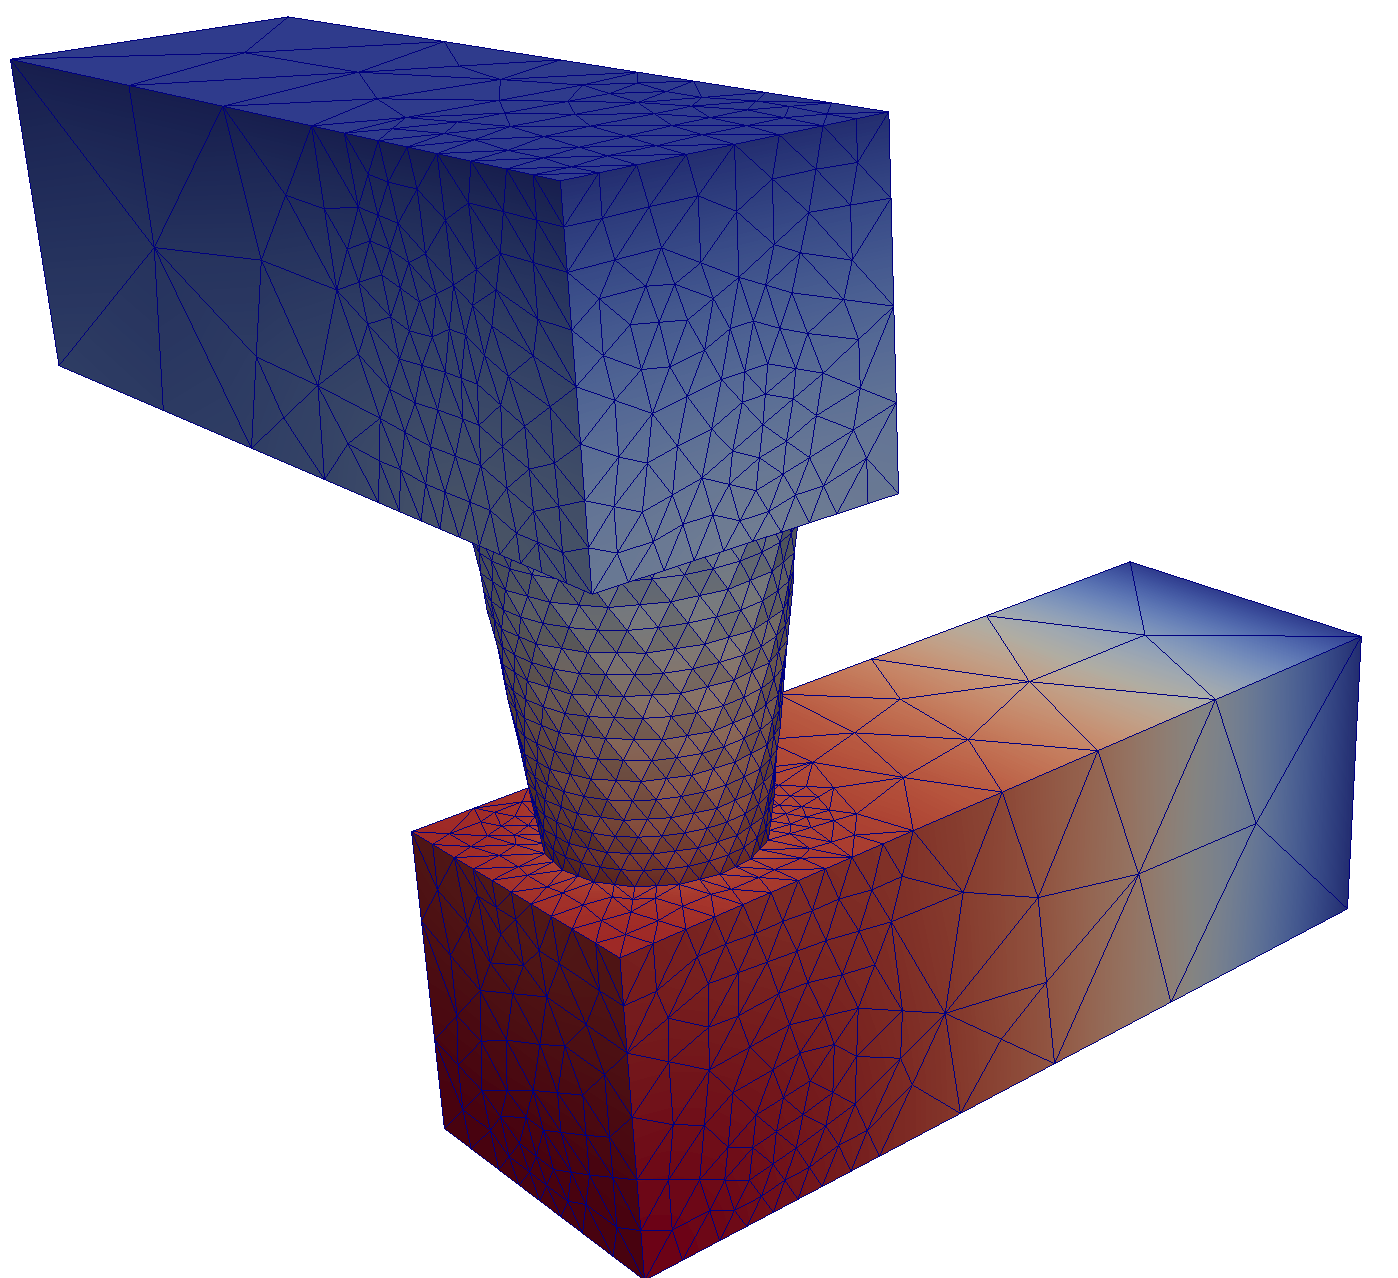
\includegraphics[width=0.47\textwidth]{sshape_3d_2}
  \end{flushright}
 \end{block}

  \vspace*{-2cm}
 \begin{block}{Work in Progress}
  \begin{itemize}
   \item PLC, hybrid meshes, multigrid
  \end{itemize}
  
 \end{block}
 %\vspace*{0.45cm}
\end{frame}









%%
%%
%%  Part 3: ViennaData
%%
%%



\begin{frame}{Contents}
  \begin{center}
   \Large Part 3: ViennaData
  \end{center}
\end{frame}

\begin{frame}{Simulation Flow}
  \begin{center}
   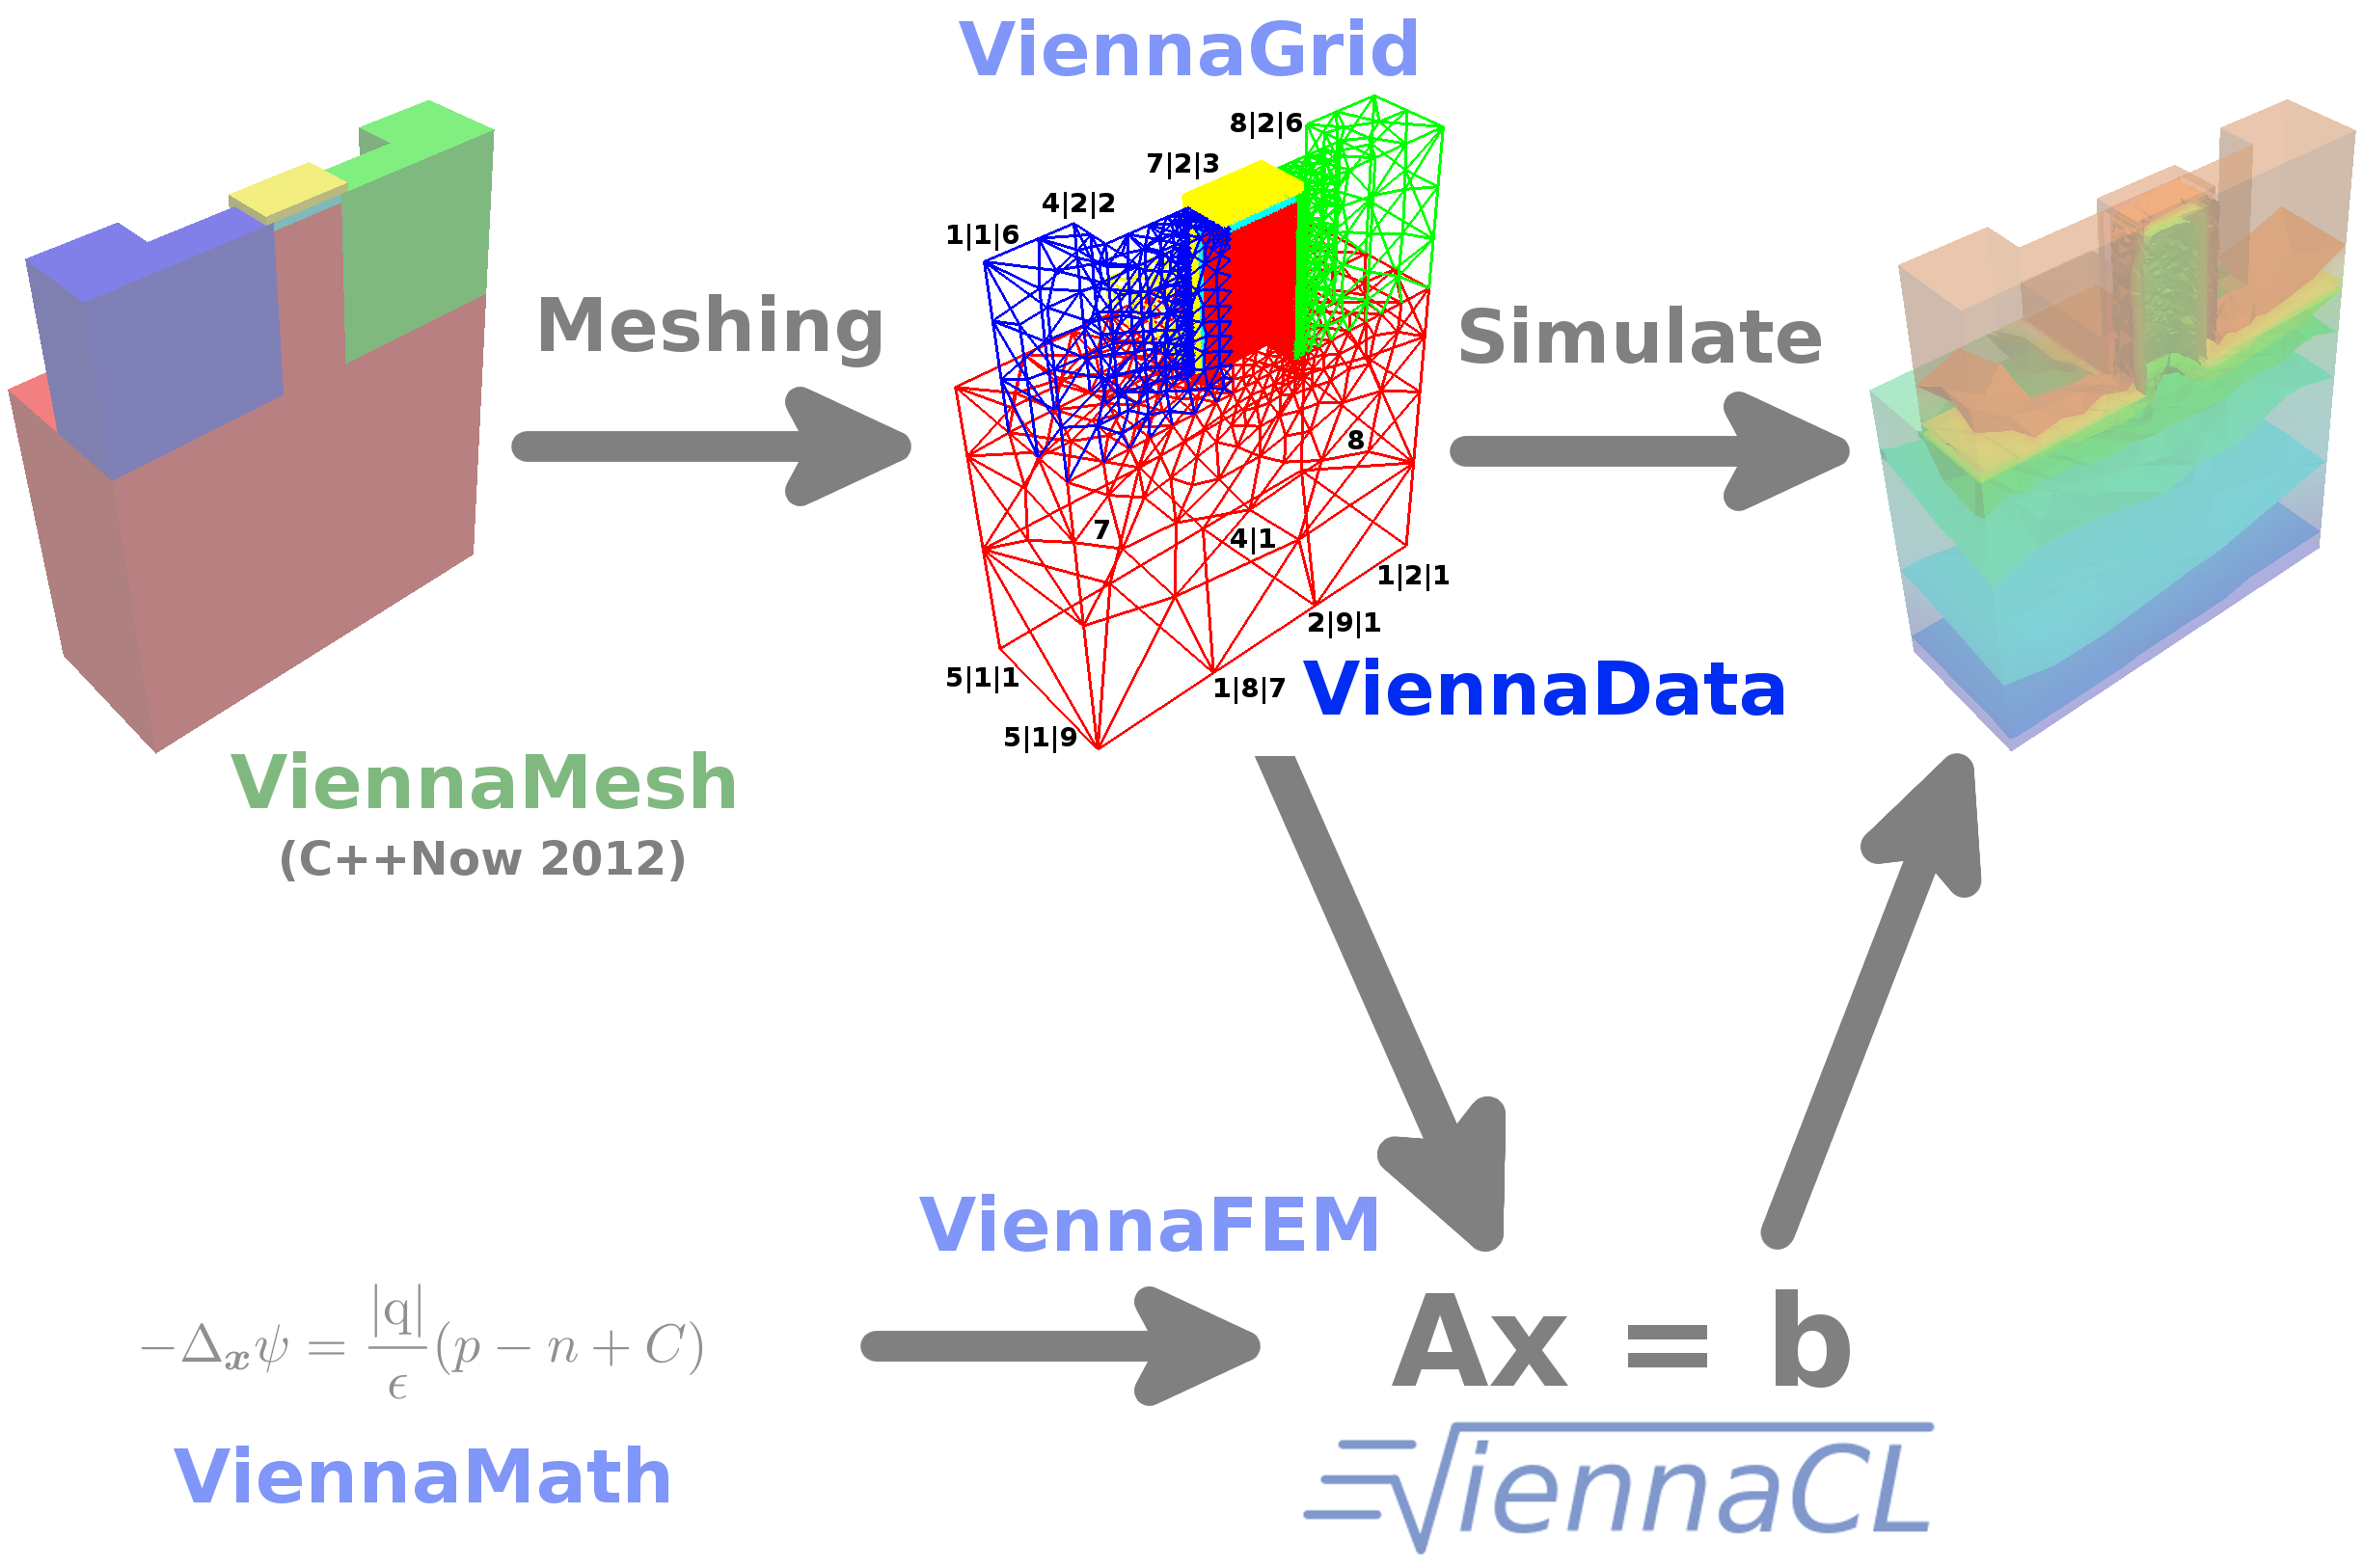
\includegraphics[width=0.99\textwidth]{flow-viennadata-2.png}
  \end{center}
\end{frame}





\begin{frame}[fragile]{Data Storage}
   
 \begin{block}{Plain Object-Oriented Approach?}
  \begin{lstlisting}
  struct Triangle {
   PointType a, b, c;
   bool is_on_boudary;
   double rho; };   //e.g. specific mass
  \end{lstlisting} 
 \end{block}

 \visible<1->{
 \begin{block}{Pros and Cons}
   \begin{itemize}
    \item Data is directly stored with the object
    \item Each (!) triangle carries a boolean flag
    \item Reusability reduced $\Rightarrow$ better rename to \texttt{TriangleWithMaterial}
  \end{itemize}
 \end{block}
 }
 
 \visible<1->{
 \begin{center}
  \Huge \color{red} Monolithic, don't do this!
 \end{center}
 }
\end{frame}



%% Data storage 2
\begin{frame}[fragile]
\frametitle{Data Storage}
 \begin{block}{Store Data with Mesh:}
  \begin{lstlisting}
  class Mesh {
   vector<Triangle> triangles;
   std::map<size_t, bool>  boudary_map; //no memory wasted
   vector<double> rho_for_triangles;   };
  \end{lstlisting} 
 \end{block}

 \visible<1->{
 \begin{block}{Pros and Cons}
   \begin{itemize}
    \item \texttt{Triangle} is still reusable
    \item \texttt{Mesh} class has to handle data storage complexity
    \item Each additional data requires a change of \texttt{Mesh} class
    \item \texttt{Mesh} object has to be passed to all modules
  \end{itemize}
 \end{block}
 }
 
 \visible<1->{
 \begin{center}
  \Huge \color{red} Monolithic, don't do this!
 \end{center}
 }
\end{frame}



\begin{frame}[fragile]
\frametitle{ViennaData}

 \begin{block}{Approach by ViennaData}
  \begin{itemize}
   \item Introduction of a hidden data container
   \item  Data is stored in a map-like manner using keys
  \end{itemize}
 \end{block}

\begin{lstlisting}[basicstyle=\scriptsize\ttfamily]
  //generic interface:
  viennadata::access<KeyType, ValueType>(key)(obj);

  //boundary flag and specific mass retrieval for triangle:
  bool on_boundary = access<BoundaryKeyType, bool>(boundary_key)(triangle);
  double       rho = access<MassKeyType,   double>(    mass_key)(triangle);
\end{lstlisting} 

  \visible<1->{
  \begin{block}{Pros and Cons}
   \begin{itemize}
    \item[+] \texttt{Triangle} and \texttt{Mesh} are still reusable
    \item[+] Can be used with arbitrary objects (third-party libraries)
    \item[+] Unified interface for data access
    \item[--] Global state
   \end{itemize}
  \end{block}
  }

\end{frame}






\begin{frame}[fragile]
\frametitle{ViennaData}

 \begin{block}{Generic Interface}
\begin{lstlisting}
  viennadata::access<KeyType, ValueType>(key)(obj);
\end{lstlisting} 
 \end{block}


 \begin{block}{Default Storage Scheme}
  \begin{itemize}
   \item If nothing is known about the object:
  \end{itemize}
  
\begin{lstlisting}
  std::map<ObjectType *,
           std::map<KeyType, ValueType> >
\end{lstlisting} 

  \begin{itemize}
   \item The compiler creates such a map for each of the following:
  \end{itemize}

\begin{lstlisting}
  access<long, double>(42)(triangle);
  access<char, double>('b')(triangle);
  access<std::string, double>("mass")(triangle);
  access<std::string, double>("mass")(vertex);
\end{lstlisting} 
 \end{block}

\end{frame}










% Fast access to data: ~2-3 slides
\begin{frame}[fragile]
\frametitle{ViennaData}

 \begin{block}{Performance Considerations}
   \begin{itemize}
    \item $\mathcal{O}(\log N) + \mathcal{O}(\log K)$ access time
    \item $N$ ... objects of same type (e.g. triangles)
    \item $K$ ... keys of same type
    \item Usually too slow in a high-performance setting
   \end{itemize}
 \end{block}

 \visible<1->{
 \begin{block}{Can We Do Better?}
  \visible<1->{
  \begin{itemize}
   \item In general: No
   \item In certain situations: Yes
  \end{itemize}
  }
 \end{block}
 }
\end{frame}

%%%%%%%%%%%%%%%%%%%%%%%%%%%%%%%%%%%



\begin{frame}[fragile]
\frametitle{ViennaData}

 \begin{block}{Type-based Key Dispatch}
   \begin{itemize}
    \item Only one key per type
    \item $\mathcal{O}(\log N)$ access time
   \end{itemize}
\begin{lstlisting}
  access<mass_key, double>(mass_key())(triangle);
  
  // or:
  access<mass_key, double>()(triangle);
\end{lstlisting} 
 \end{block}

 \begin{block}{Internal Datastructure}
\begin{lstlisting}
  std::map<ObjectType *, ValueType>
\end{lstlisting} 
   \begin{itemize}
    \item Transparent to user
    \item One line of code for activation
   \end{itemize}
 \end{block}
\end{frame}


%%%%%%%%%%%%%%%%%%%%%%%%%%



\begin{frame}[fragile]
\frametitle{ViennaData}

 \begin{block}{Numeric IDs for Objects}
   \begin{itemize}
    \item Only one key per type
    \item $\mathcal{O}(K)$ access time
    \item $\mathcal{O}(1)$ access time with type-based key dispatch
   \end{itemize}
 \end{block}
\begin{lstlisting}
  access<std::string, double>("mass")(triangle);
  
  // with type-based key dispatch:
  access<mass_key, double>()(triangle);
\end{lstlisting} 

 \begin{block}{Internal Datastructure}
\begin{lstlisting}
  std::vector<ValueType>
\end{lstlisting} 
   \begin{itemize}
    \item Transparent to user
    \item One line of code for activation
    \item Overload generic \lstinline|id()| accessor
   \end{itemize}
 \end{block}
\end{frame}



% Benchmark from manual: ~2 slides


\begin{frame}[fragile]
 \frametitle{ViennaData}

 \begin{block}{Benchmarking ViennaData}
   \begin{itemize}
    \item ID-based access to data via ViennaData (class \lstinline|LightWeight|)
    \item OOP-style storage in classes with payload
   \end{itemize}
 
 \begin{lstlisting}
   template <size_t N>
   struct FatClass {
     double data;
     char payload[N];
   };
 \end{lstlisting}

 \end{block}

 \visible<1->{
  \begin{center}
  \begin{tabular}{|l|c|c|}
 \hline
        &  $10^3$ Objects (us) & $10^6$ Objects (ms) \\
 \hline
 \lstinline|LightWeight|    & \textbf{4} & \textbf{5} \\
 \lstinline|FatClass<10>|   & \textbf{1.3} & \textbf{4} \\
 \lstinline|FatClass<100>|  & 2.1 & 11 \\
 \lstinline|FatClass<1000>| & 2.5 & 11 \\
 \hline
 \end{tabular}
  \end{center}
 }
\end{frame}






\begin{frame}[fragile]
 \frametitle{ViennaData}

 \begin{block}{Other Routines}
  \begin{itemize}
   \item Not further addressed:
 \begin{lstlisting}
  viennadata::copy<KeyType, ValueType>(key)(src_obj, dst_obj);
  viennadata::move<KeyType, ValueType>(key)(src_obj, dst_obj);
  viennadata::find<KeyType, ValueType>(key)(obj);
  
  viennadata::erase<KeyType, ValueType>(key)(obj);
  viennadata::erase<KeyType, all>(key)(obj);  
  viennadata::erase<all, ValueType>(key)(obj);  
 \end{lstlisting}
  \end{itemize}
 \end{block}

  \visible<1->{
  \begin{block}{Pitfalls}
   \begin{itemize}
    \item Inheritance
    \item Limited lifetime of objects
    \item Compilation units with different configuration
   \end{itemize}
  \end{block}
  }

\end{frame}







%%
%%
%%  Part 4: ViennaMath
%%
%%




\begin{frame}{Contents}
  \begin{center}
   \Large Part 4: ViennaMath
  \end{center}
\end{frame}

\begin{frame}{Simulation Flow}
  \begin{center}
   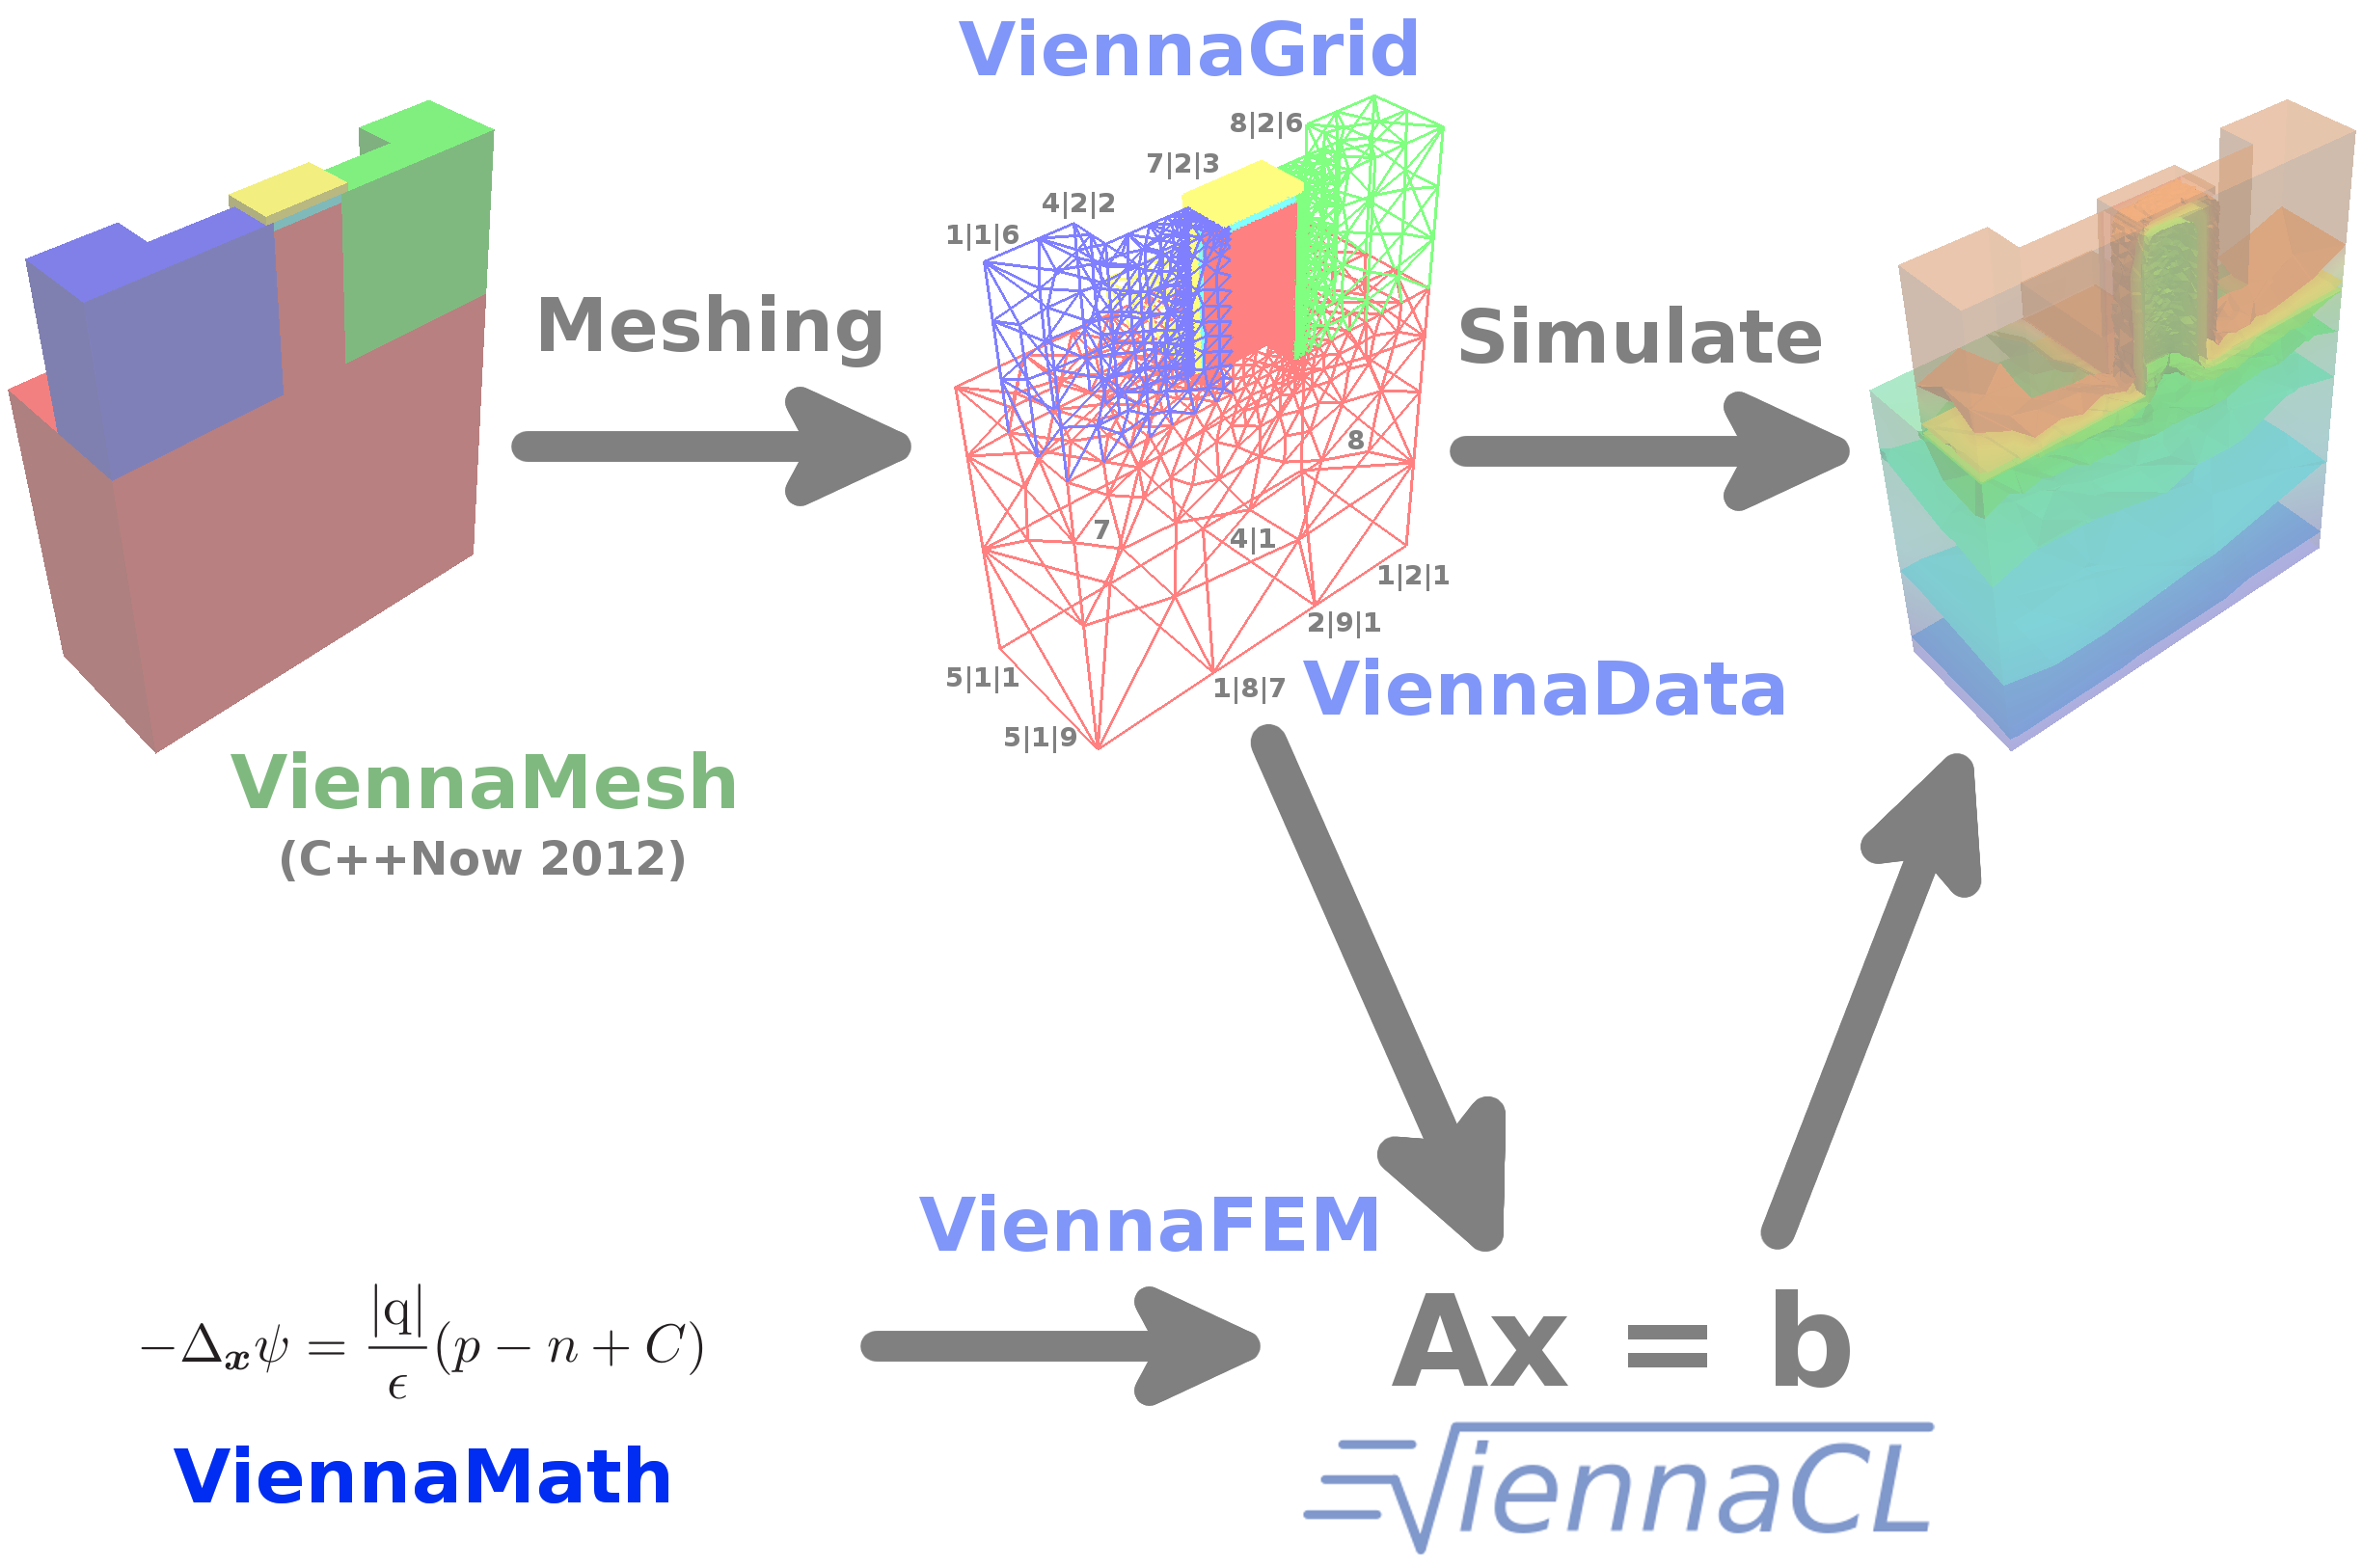
\includegraphics[width=0.99\textwidth]{flow-viennamath-2.png}
  \end{center}
\end{frame}


%%%%%% Expected talk time: 15 minutes, ~7 slides



\begin{frame}[fragile]
\frametitle{ViennaMath}

 \begin{block}{A Symbolic Math Library in C++}
   \begin{itemize}
    \item Symbolic evaluation and manipulation of math expressions
    \item Unified run time and compile time interface
    \item Differentiation and integration provided
    \item {\LaTeX} output
   \end{itemize}
 \end{block}

 \begin{block}{Example Usage}
\begin{lstlisting}
  variable x(0);
  variable y(1);
  variable z(2);
  expr f = x + y - z;
  expr g = f * f;
  eval(f, make_vector(1.0, 2.0, 4.0)); // returns -1.0
  eval(g, make_vector(1.0, 2.0, 4.0)); // returns  1.0
\end{lstlisting} 
   \begin{itemize}
    \item Run Time Evaluation
   \end{itemize}
 \end{block}
\end{frame}



%%%%%%%%%%%%%%%%%%%%%

\begin{frame}[fragile]
\frametitle{ViennaMath}

 \begin{block}{A Symbolic Math Library in C++}
   \begin{itemize}
    \item Symbolic evaluation and manipulation of math expressions
    \item Unified run time and compile time interface
    \item Differentiation and integration provided
    \item {\LaTeX} output
   \end{itemize}
 \end{block}

 \begin{block}{Example Usage}
\begin{lstlisting}
  ct_variable<0> x;
  ct_variable<1> y;
  ct_variable<2> z;
  ct_constant<1> c1;
  ct_constant<2> c2;
  ct_constant<4> c4;
  eval(x + y - z, make_vector(c1, c2, c4)); // returns -1
\end{lstlisting} 
   \begin{itemize}
    \item Compile Time Evaluation
   \end{itemize}
   \vspace*{-0.05cm}
 \end{block}
\end{frame}

%%%%%%%%%%%%%%%%%%%%%%%%%%%%%%%%%



\begin{frame}[fragile]
\frametitle{ViennaMath}

 \begin{block}{Substitution and Differentiation (Run Time)}
\begin{lstlisting}
  variable x(0);
  variable y(1);
  variable z(2);
  substitute(x, y, x*y + z); // returns y*y+z
  diff(x*y + z, x);          // returns y
\end{lstlisting} 
 \end{block}
 
 \begin{block}{Substitution and Differentiation (Compile Time)}
\begin{lstlisting}
  ct_variable<0> x;
  ct_variable<1> y;
  ct_variable<2> z;
  substitute(x, y, x*y + z); // returns y*y+z
  diff(x*y + z, x);          // returns y
\end{lstlisting} 
 \end{block}
 
\end{frame}

%%%%%%%%%%%%%%%%%%%%%%%%%%%%%%%%


\begin{frame}[fragile]
\frametitle{ViennaMath}

 \begin{block}{Numerical Integration (Run Time): $\color{black} \int_0^1 x^2 \: \mathrm{d} x$}
\begin{lstlisting}
  expr f = integral( make_interval(0, 1), x*x, x );

  numerical_quadrature integrator(new gauss_quad_1());
  integrator(f);                             // method 1
  integrator(make_interval(0, 1), x*x, x);   // method 2
\end{lstlisting} 
 \end{block}
 
 \begin{block}{Analytical Integration (Compile Time): {\color{black} $\int_0^1 x^2 \: \mathrm{d} x$, $\int_0^1 \int_0^{1-x} xy \: \mathrm{d}x \mathrm{d}y$} }
\begin{lstlisting}
  integrate(make_interval(c0, c1),
            x*y,
            x );    //returns y/2.0
  integrate(make_interval(c0, c1),
            integrate( make_interval(c0, c1 - x), x*y, y),
            x);    //returns 1.0/24.0
\end{lstlisting} 
 \end{block}
 
\end{frame}

%%%%%%%%%%%%%%%%%%%%%%%%%%%%%%%%


\begin{frame}[fragile]
\frametitle{ViennaMath}

 \begin{block}{Function Symbols}
   \begin{itemize}
    \item Represent a function (not evaluable)
   \end{itemize}
 \end{block}

 \begin{block}{Differential Operators}
   \begin{itemize}
    \item Gradient, Divergence
   \end{itemize}
 \end{block}

 \begin{block}{Symbolic Integration Domain}
   \begin{itemize}
    \item Specify actual integration domain and integration variables \emph{later}
   \end{itemize}
 \end{block}
 
\begin{lstlisting}
  function_symbol u;
  equation eq( laplace(u), 1.0 );  // Poisson equation
  
  function_symbol v;
  expr w = integral(symbolic_interval(),
                    grad(u) * grad(v));
\end{lstlisting} 
 
\end{frame}



% Maybe throw in one or two more slides




%%
%%
%%  Part 4: ViennaFEM
%%
%%




\begin{frame}{Contents}
  \begin{center}
   \Large Part 5: ViennaFEM
  \end{center}
\end{frame}


\begin{frame}{Simulation Flow}
  \begin{center}
   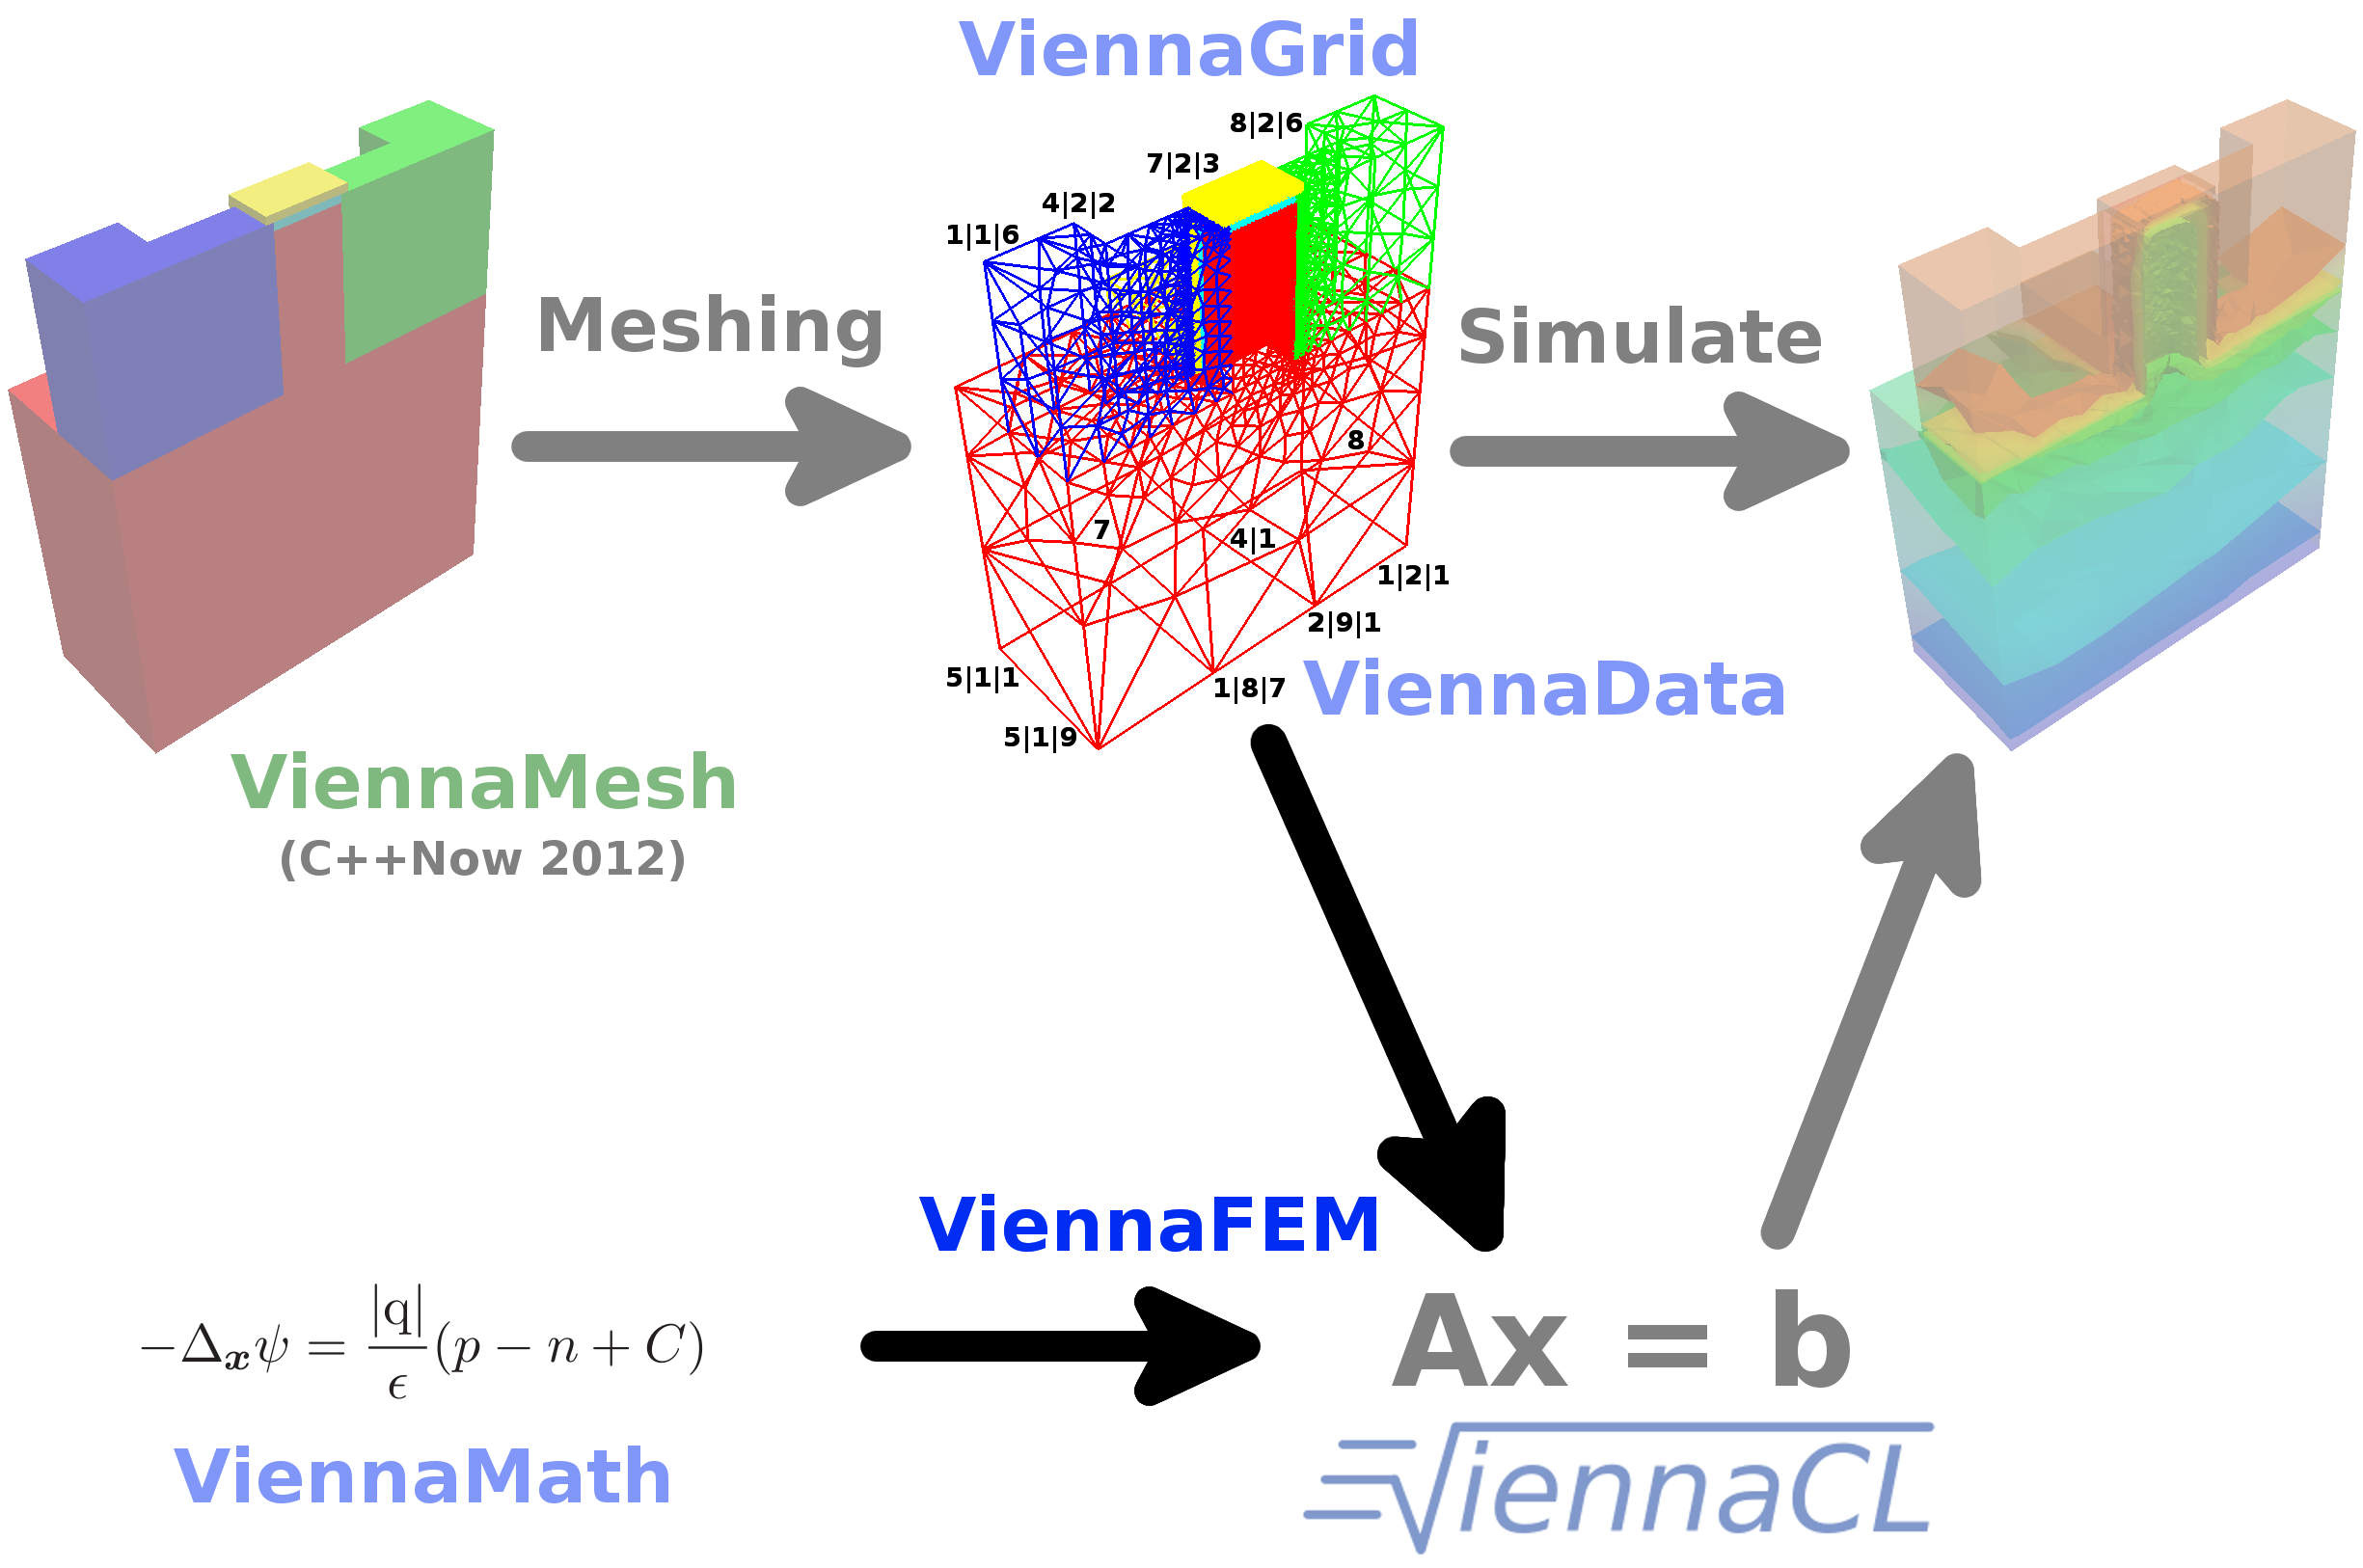
\includegraphics[width=0.99\textwidth]{flow-viennafem-2.png}
  \end{center}
\end{frame}


%%%%%% Expected talk time: 10 minutes, ~5 slides  (maybe with backup slides)


\begin{frame}{Simulation Flow}

  \begin{center}
   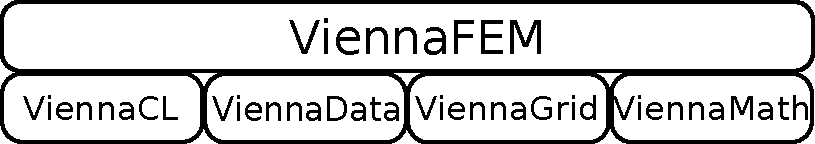
\includegraphics[width=0.6\textwidth]{ViennaFEM-arch.pdf}
  \end{center}
 \begin{block}{Library-Centric Design}
  \begin{itemize}
   \item ViennaCL for linear solver
   \item ViennaData for data storage
   \item ViennaGrid for mesh handling
   \item ViennaMath for symbolic math
  \end{itemize}
 \end{block}
 
 \visible<1->{
 \begin{block}{Addresses Come\&Go in Academia}
  \begin{itemize}
   \item Focus on one package
   \item No in-depth knowledge of all packages required
   \item Additional emphasis on good interfaces
  \end{itemize}
 \end{block}
 }
 
\end{frame}

%%%%%%%%%%%%%%%%%%%%%%%5



\begin{frame}[fragile]
\frametitle{ViennaFEM}

\begin{block}{ViennaGrid deals with the Mesh}
\begin{lstlisting}[basicstyle=\scriptsize\ttfamily]
DomainType my_domain;
viennagrid::io::netgen_reader my_reader;
my_reader(my_domain, "mystructure.mesh");
\end{lstlisting}
\end{block}

\begin{block}{Equation specification via ViennaMath: $\color{black} \Delta u = -1$}
\begin{lstlisting}[basicstyle=\scriptsize\ttfamily]
equation poisson_eq = viennamath::make_equation(laplace(u), -1);
\end{lstlisting}
\end{block}


\begin{block}{Assembly via ViennaFEM}
\begin{lstlisting}[basicstyle=\scriptsize\ttfamily]
viennafem::pde_assembler fem_assembler;
fem_assembler(viennafem::make_linear_pde_system(poisson_eq, u),
              my_domain,
              system_matrix, load_vector);
\end{lstlisting}
\end{block}

\begin{block}{Linear solver provided by ViennaCL}
\begin{lstlisting}[basicstyle=\scriptsize\ttfamily]
VectorType pde_result 
  = viennacl::linalg::solve(system_matrix, load_vector, cg_tag());
\end{lstlisting}
\end{block}
 
\end{frame}


%%%%%%%%%%%%%%%%%%%%%%%

\begin{frame}[fragile]
\frametitle{ViennaFEM}

 \begin{block}{Lame equation for Linear Elasticity}

  \begin{align*} 
    \int_\Omega \varepsilon(u) : \sigma(v) \: \mathrm{d} \Omega =
    \int_\Omega F \cdot v \: \mathrm{d} \Omega \quad \forall v \in \mathcal{V}
  \end{align*}

   \begin{itemize}
    \item With $F = (0, 0, 1)^{\mathrm{T}}$:
   \end{itemize}
   
  \begin{lstlisting}
  std::vector< Expression > strain = strain_tensor(u);
  std::vector< Expression > stress = stress_tensor(v);
  
  Equation weak_form_lame = make_equation(
             integral(symbolic_interval(),
                      tensor_reduce( strain, stress )),
             //=                                         
             integral(symbolic_interval(),
                      constant(1.0) * v[2])
                                         );
  \end{lstlisting}
   

 \end{block}

\end{frame}

\begin{frame}{Solving Lame's Equation for a TSV}
 \begin{center}
  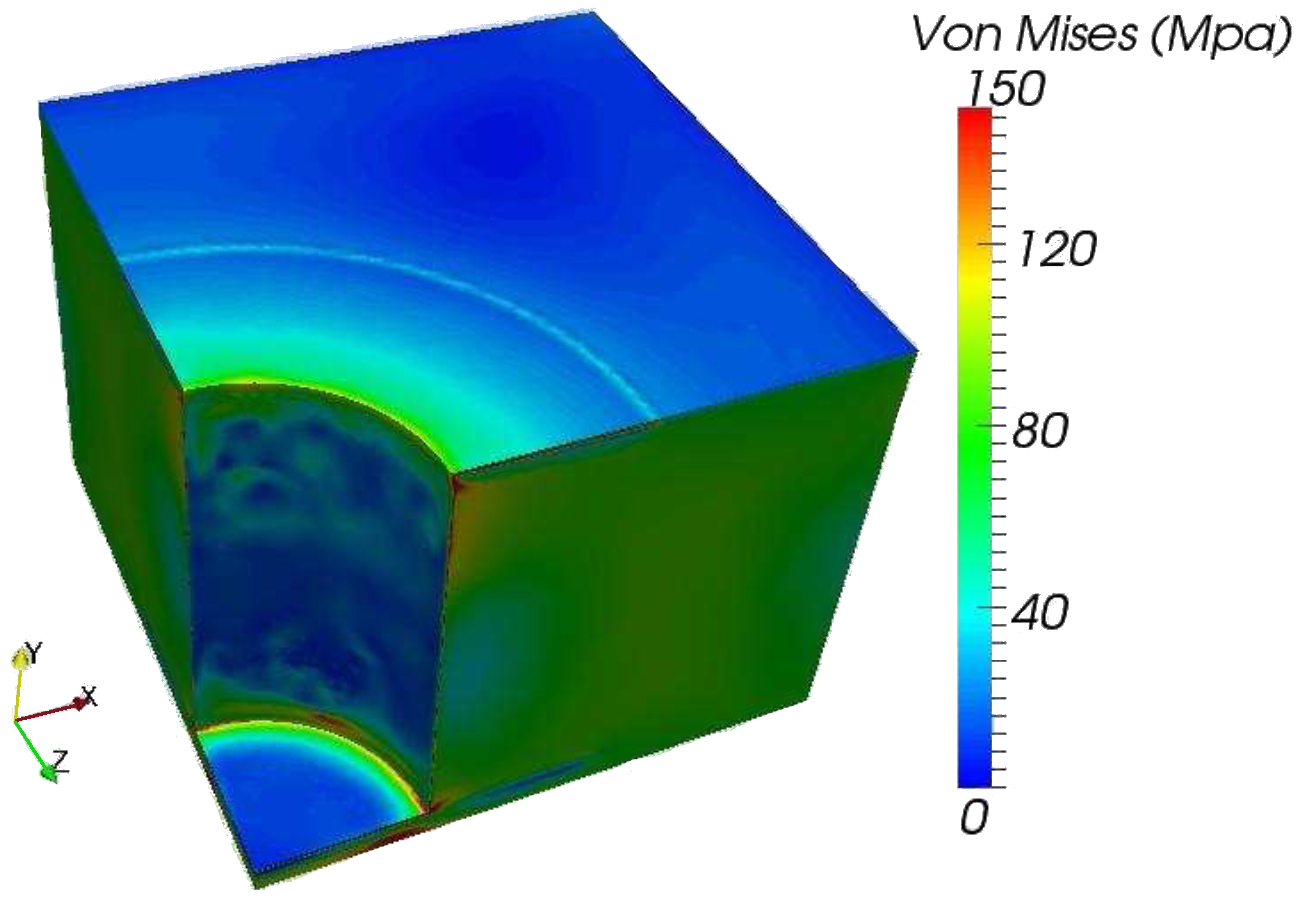
\includegraphics[width=0.8\textwidth]{figures/tsv.png}
 \end{center}
\end{frame}







\begin{frame}{Summary}

  \begin{block}{Software Packages}
   \begin{itemize}
    \item ViennaCL:   \hspace*{0.50cm} GPU-accelerated Linear Algebra
    \item ViennaData: \hspace*{0.19cm} Generic Data Storage 
    \item ViennaFEM:  \hspace*{0.23cm} Modular High-Level Finite Element Package
    \item ViennaGrid: \hspace*{0.27cm} Generic Mesh Datastructure
    \item ViennaMath: \hspace*{0.17cm} Symbolic Math Kernel
   \end{itemize}

   \begin{center}
     \ttfamily http://vienna\{cl,data,fem,grid,math\}@sourceforge.net
   \end{center}

  \end{block}

  \begin{block}{Design Philosophy}
   \begin{itemize}
    \item Orthogonal Software Design
    \item Convenient High-Level User API
    \item Avoid Unneeded Dependencies
    \item Free Open Source (MIT License)
   \end{itemize}
  \end{block}

\end{frame}



\end{document}

